\documentclass[11pt,a4paper,openright,oneside,titlepage,fleqn,%
               headinclude,footinclude,BCOR5mm,%
               numbers=noenddot,cleardoublepage=empty,%
               tablecaptionabove]{scrreprt}
             
\usepackage[ngerman]{babel}
\usepackage[ansinew]{inputenc}
\usepackage[T1]{fontenc}
%usepackae[final]{microtype}
%\usepackage{amsmath,amssymb,amsthm}
\usepackage{varioref}
\usepackage[style=philosophy-modern,backend=bibtex8,hyperref,square,natbib,ibidtracker=false]{biblatex}
\usepackage{chngpage}
\usepackage{mflogo}
\usepackage{caption,listings,graphicx,subfig}
\usepackage{calc}
\usepackage{listings}
\usepackage{wrapfig}
\usepackage{subfig}
\usepackage{multicol}
\usepackage{makeidx}
\usepackage{fixltx2e}
\usepackage{xspace}
\usepackage{relsize}
\usepackage{mparhack}
\usepackage[eulerchapternumbers,subfig,beramono,eulermath,pdfspacing,listings, dottedtoc]{classicthesis}
\usepackage{arsclassica}
\usepackage{xcolor}
\usepackage{tikz}
\usepackage{framed}
\usepackage{guit}
\usepackage[margin=1.4in, a4paper]{geometry}
\usepackage{wrapfig}
% ********************************************************************
% arsclassica-settings
% ********************************************************************



\newcommand{\myName}{Stefan Schneider}
\newcommand{\myTitle}{Street Art}
\newcommand{\mySubTitle}{Zwischen Kunst und Kommerz}
\newcommand{\myLocation}{Pfeffingen}
\newcommand{\myGroup}{Klasse 3Wa}
\newcommand{\myUrl}{Betreut von: Heike M�ller}
\newcommand{\mySchools}{Gymnasium M�nchenstein}
\newcommand{\myTime}{2012, April}

% ********************************************************************
% page layout
% ******************************************************************** 
\marginparwidth 200pt
\parindent 0pt
\parskip 1ex
\renewcommand{\baselinestretch}{1.25}

% ********************************************************************
% hyperref
% ******************************************************************** 
\newcommand{\mail}[1]{\href{mailto:#1}{\texttt{#1}}}


% ********************************************************************
% makeidx, multicol
% ********************************************************************
\let\orgtheindex\theindex
\let\orgendtheindex\endtheindex
\def\theindex{%
	\def\twocolumn{\begin{multicols}{2}}%
	\def\onecolumn{}%
	\clearpage
	\orgtheindex
}
\def\endtheindex{%
	\end{multicols}%
	\orgendtheindex
}

\makeindex


% ********************************************************************
% listings
% ********************************************************************

\definecolor{lightergray}{gray}{0.99}

\lstset{language=[LaTeX]Tex,
    keywordstyle=\color{RoyalBlue},
    basicstyle=\normalfont\ttfamily,
    commentstyle=\color{Emerald}\ttfamily,
    stringstyle=\rmfamily,
    numbers=none,
    numberstyle=\scriptsize,
    stepnumber=5,
    numbersep=8pt,
    showstringspaces=false,
    breaklines=true,
    frameround=ftff,
    frame=lines,
    backgroundcolor=\color{lightergray}
} 

\lstset{	morekeywords=%
        {RequirePackage,newboolean,DeclareOption,setboolean,%
        ProcessOptions,PackageError,ifthenelse,boolean,%
        chapterNumber,sodef,textls,allcapsspacing,%
        MakeTextLowercase,orgtheindex,endtheindex,%
        @ifpackageloaded,undefined,sfdefault,%
        DeclareRobustCommand,spacedallcaps,%
        microtypesetup,MakeTextUppercase,lowsmallcapsspacing,%
        lowsmallcapsspacing,spacedlowsmallcaps,
        spacedlowsmallcaps,lehead,headmark,color,%
        headfont,partname,thepart,titleformat,part,
        titlerule,chapter,thechapter,thesection,%
        subsection,thesubsection,thesubsubsection,%
        paragraph,theparagraph,descriptionlabel,titlespacing,%
        graffito,lineskiplimit,finalhyphendemerits,%
        colorbox,captionsetup,labelitemi,%
        myincludegraphics,hypersetup,setlength,%
        definecolor,lsstyle,textssc,subsubsection,%
        graffito@setup,includegraphics,ifdefined,%
        myTitle,textcopyright,myName,lstset,lstnewenvironment,%
        setkeys,lst@BeginAlsoWriteFile,contentsname,%
        toc@heading,@ppljLaTeX,z@,check@mathfonts,%
        sf@size,ptctitle,mtctitle,stctitle,lst@intname,%
        @empty,math@fontsfalse,@ppljscTeX,@iwonaTeX,%
        @iwonascLaTeX,@ctTeX,tw@,ct@sc,@ctTeX,f@family,%
        f@shape,ct@sc,ctLaTeX,ctLaTeXe,@twoe,@sctwoe,%
        texorpdfstring,m@th,ctTeX,@mkboth,ProvidesPackage,%
        theindex,PackageInfo,PackageWarningNoLine,%
        mtifont,mtcindent,@iwonaLaTeX,@ppljTeX,@iwonascTeX,%
        rohead,orgendtheindex,@ppljscLaTeX,%
        @ifclassloaded,toc@headingbkORrp,backreftwosep,%
        backrefalt,backreflastsep,areaset,pnumfont,%
        arsincludegraphics,ExecuteOptions,PackageWarning,textcolor,%
        MessageBreak,ars@@includegraphics,ifcld@backref,rofoot,formatchapter,%
        if@twoside},
        commentstyle=\color{Emerald}\ttfamily,%
        frame=lines}

\lstset{basicstyle=\normalfont\ttfamily}
\lstset{flexiblecolumns=true}
\lstset{moredelim={[is][\normalfont\itshape]{/*}{*/}}}
\lstset{basicstyle=\normalfont\ttfamily}
\lstset{flexiblecolumns=false}
\lstset{moredelim={[is][\ttfamily]{!?}{?!}}} 
\lstset{escapeinside={�*}{*�}}
\lstset{firstnumber=last}
\lstset{moredelim={[is][\ttfamily]{!?}{?!}}}

\DeclareRobustCommand*{\pacchetto}[1]{{\normalfont\ttfamily#1}%
\index{Pacchetto!#1@\texttt{#1}}%
\index{#1@\texttt{#1}}}

\DeclareRobustCommand*{\bibtex}{\textsc{Bib}\TeX%
\index{bibtex@\textsc{Bib}\protect\TeX}%
}

\DeclareRobustCommand*{\amseuler}{\protect\AmS{} Euler%
\index{AmS Euler@\protect\AmS~Euler}%
\index{Font!AmS Euler@\protect\AmS~Euler}}

\lstnewenvironment{code}% 
{\setkeys{lst}{columns=fullflexible,keepspaces=true}%
\lstset{basicstyle=\small\ttfamily}%
}{}

\lstset{extendedchars} 
\lstnewenvironment{sidebyside}{% 
    \global\let\lst@intname\@empty 
    \setbox\z@=\hbox\bgroup 
    \setkeys{lst}{columns=fullflexible,% 
    linewidth=0.45\linewidth,keepspaces=true,%
    breaklines=true,% 
    breakindent=0pt,%
    boxpos=t,%
    basicstyle=\small\ttfamily
}% 
    \lst@BeginAlsoWriteFile{\jobname.tmp}% 
}{% 
    \lst@EndWriteFile\egroup 
        \begin{center}% 
            \begin{minipage}{0.45\linewidth}% 
                \hbox to\linewidth{\box\z@\hss} 
            \end{minipage}% 
            \qquad 
            \begin{minipage}{0.45\linewidth}%
            \setkeys{lst}{frame=none}% 
                \leavevmode \catcode`\^^M=5\relax 
                \small\input{\jobname.tmp}% 
            \end{minipage}% 
        \end{center}% 
} 

\newcommand{\omissis}{[\dots\negthinspace]}

\graphicspath{{Graphics/}}

\hyphenation{Robert Bring-hurst DejaVu
Bera Mono Vera Classic-Thesis suite Knuth Zapf}

\newcommand{\meta}[1]{$\langle${\normalfont\itshape#1}$\rangle$}
\lstset{escapeinside={�*}{*�}}


\DeclareRobustCommand*{\miktex}{MiK\TeX%
\index{miktex@MiK\protect\TeX}%
}

\DeclareRobustCommand*{\metafont}{\MF%
\index{METAFONT@\protect\MF}%
}

\DeclareRobustCommand*{\metapost}{\MP%
\index{METAPOST@\protect\MP}%
}

\DeclareRobustCommand*{\texlive}{\TeX{}~Live%
\index{texlive@\protect\TeX{}~Live}%
}


% ********************************************************************
% biblatex
% ******************************************************************** 

\bibliography{Bibliography}

\renewcommand{\nameyeardelim}{, }

\defbibheading{bibliography}{%
\cleardoublepage
\manualmark
\phantomsection
\addcontentsline{toc}{chapter}{\tocEntry{\bibname}}
\chapter*{\bibname\markboth{\spacedlowsmallcaps{\bibname}}
{\spacedlowsmallcaps{\bibname}}}}     

  \DeclareCiteCommand{\citeyearpar}[\mkbibparens] 
  {\boolfalse{citetracker}% 
   \boolfalse{pagetracker}% 
   \usebibmacro{prenote}} 
  {\printtext[bibhyperref]{\printfield{year}}} 
  {\multicitedelim} 
  {\usebibmacro{postnote}} 

\makeatletter 
  \DeclareCiteCommand{\citetalias} 
  {\usebibmacro{prenote}} 
  {\usebibmacro{citeindex}% 
   \bibhyperref{\@citealias{\thefield{entrykey}}}} 
  {\multicitedelim} 
  {\usebibmacro{postnote}} 
\makeatother 

\setcounter{biburlnumpenalty}{9000}
\setcounter{biburlucpenalty}{9000}
\setcounter{biburllcpenalty}{9000}


% ********************************************************************
% other commands
% ******************************************************************** 

\newcommand{\ita}[1]{% 
  \begin{otherlanguage*}{italian}#1\end{otherlanguage*}}
  
\DeclareRobustCommand*{\pkgname}[1]{{\normalfont\sffamily#1}%
\index{Package!#1@\textsf{#1}}%
\index{#1@\textsf{#1}}}

\DeclareRobustCommand*{\envname}[1]{{\normalfont\ttfamily#1}%
\index{Environment!#1@\texttt{#1}}%
\index{#1@\texttt{#1}}}

\DeclareRobustCommand*{\optname}[1]{{\normalfont\ttfamily#1}%
\index{Option!#1@\texttt{#1}}%
\index{#1@\texttt{#1}}}

\DeclareRobustCommand*{\clsname}[1]{{\normalfont\sffamily#1}%
\index{Class!#1@\textsf{#1}}%
\index{#1@\textsf{#1}}}

\DeclareRobustCommand*{\cmdname}[1]{\mbox{\lstinline!\\#1!}%
\index{#1@\texttt{\hspace*{-1.2ex}\textbackslash#1}}}

\DeclareRobustCommand*{\classicthesis}{Classic\-Thesis}

\DeclareRobustCommand*{\arsclassica}{{\normalfont\sffamily ArsClassica}}

\DeclareRobustCommand*{\miktex}{MiK\TeX%
\index{miktex@MiK\protect\TeX}}

\DeclareRobustCommand*{\texlive}{\TeX{}~Live%
\index{texlive@\protect\TeX{}~Live}}



% ********************************************************************
% Quotes
% ******************************************************************** 

% Make commands for the quotes
\newcommand*{\openquote}{\tikz[remember picture,overlay,xshift=-15pt,yshift=-10pt]
     \node (OQ) {\quotefont\fontsize{60}{60}\selectfont``};\kern0pt}
\newcommand*{\closequote}{\tikz[remember picture,overlay,xshift=15pt,yshift=10pt]
     \node (CQ) {\quotefont\fontsize{60}{60}\selectfont''};}
% select a colour for the shading
\definecolor{shadecolor}{named}{lightergray}
% wrap everything in its own environment
\newenvironment{shadequote}%
{\begin{snugshade}\begin{quote}\openquote}
{\hfill\closequote\end{quote}\end{snugshade}}





%\setlength{\emgencystretch}{1em}


\begin{document}
%\begin{flushleft}
%\selectlanguage{ngerman}
\pagenumbering{arabic}
\pagestyle{plain}
%******************************************************************
% Frontmatter
%******************************************************************
\begin{titlepage}
\pdfbookmark{Titelblatt}{Titelblatt}
\changetext{}{}{}{((\paperwidth  - \textwidth) / 2) - \oddsidemargin - \hoffset - 1in}{}
\null\vfill
\begin{center}
\large
\sffamily

\bigskip

{\Large\spacedlowsmallcaps{\myName}} \\

\bigskip

{\huge\spacedlowsmallcaps{\myTitle} \\
}

\bigskip
    
\vspace{9cm}

\begin{tabular} {cc}
\parbox{0.3\textwidth}{
\includegraphics[width=4cm]{Graphics/rat2}}
&
\parbox{0.7\textwidth}{{\Large\spacedlowsmallcaps{\mySubTitle}} \\ 

					{\normalsize
					
					\myGroup \\
					\myUrl \\
					\mySchools \\
					\myTime}}
			\end{tabular}
\end{center}
\vfill
\end{titlepage}




\input{FrontBackMatter/Titelr�ckseite}
\clearpage
%*******************************************************
% Contents
%*******************************************************
\phantomsection
\pdfbookmark{\contentsname}{tableofcontents}
\setcounter{tocdepth}{2}
\begingroup 
    \let\clearpage\relax
    \let\cleardoublepage\relax

    \tableofcontents
\endgroup
\markboth{\spacedlowsmallcaps{\contentsname}}{\spacedlowsmallcaps{\contentsname}} 

\begingroup 
    \let\clearpage\relax
    \let\cleardoublepage\relax
\endgroup

\clearpage


%*******************************************************
% Abstract
%*******************************************************

%\pdfbookmark{Abstract}{Abstract}
\begingroup
\let\clearpage\relax
\let\cleardoublepage\relax
\let\cleardoublepage\relax
\phantomsection
\addcontentsline{toc}{chapter}{\tocEntry{Abstract}}
%\addcontentsline{toc}{chapter}{\smallcaps{Abstract}}
\chapter*{Abstract}
In meiner Arbeit er�rtere ich, wo Street-Art auf dem Weg in die �ffentlichen Galerien und Museen steht und inwiefern Street-Art als hochkulturelle Kunstform vom etablierten Kunstbetrieb anerkannt ist.\\
Ich bin an diese Fragestellung mit intensiver Recherche von kunststhistorischen und soziokulturellen B�cher und Artikeln herangegangen. Die Ergebnisse habe ich mit Interviews von Street-Art-K�nstlern untermauert.
Ich bin zum Schluss gekommen, dass Street-Art noch nicht von der etablierten Kunstwelt anerkannt ist und es f�r viele Street-Art-K�nstler aufgrund ihrer fehlenden kunsthistorischen Ausbildung schwierig ist, sich auf dem kommerziellen Kunstmarkt zu behaupten.\\
Die Street-Art-Szene befindet sich jedoch in stetigem Wandel und es bleibt abzuwarten, wie sich die Situation in naher Zukunft entwickeln wird, denn die Street-Art-Bewegung beherbergt grosses k�nstlerisches Potential.\\
\endgroup			
\vfill
\clearpage
\vfill


%*******************************************************
% Vorwort
%*******************************************************

%\pdfbookmark{Vorwort}{Vorwort}
\begingroup
\let\clearpage\relax
\let\cleardoublepage\relax
\let\cleardoublepage\relax
\phantomsection
\addcontentsline{toc}{chapter}{\tocEntry{Vorwort}}
%\addcontentsline{toc}{chapter}{\smallcaps{Vorwort}}
\chapter*{Vorwort}
Schon als kleiner Junge betrachtete ich im Tram oder im Zug beim Vorbeifahren gerne die bunten Graffiti und Malereien an den W�nden.
Ich wunderte mich schon damals wer denn das dorhin malt, und was die mysteri�sen Schriftz�ge denn eigentlich bedeuteten.
\\%%
Etwas sp�ter interessierte ich mich immer mehr f�r diese "`Wandmalereien"'. Ich besuchte Street-Art-Vernissagen und lernte selbst einige K�nstler kennen.
Mit diesen Bekanntschaften kam auch immer wieder die Frage auf, ob man denn seine auch Kunst verkaufen kann oder will. Viele Street-Art-K�nstler sehen dem mit gemischten Gef�hlen entgegen. 
\\
In letzter Zeit erzielten Street-Art-Werke immer wieder erstaunliche Preise\footnote{Banksys "`Bombing Middle England"' z.B wurde f�r 100'000 Pfund versteigert} auf dem Kunstmarkt und da fragte ich mich, wie es denn allgemein in der Street-Art-Szene aussieht in Sachen kommerzielle Arbeiten und Verkauf von Werken. Dies f�hrte dann zur Fragestellung meiner Maturarbeit: Wo befindet sich Street-Art auf dem Weg in Galerien und Museen?
\endgroup			


%*******************************************************
% Danksagugnen
%*******************************************************
\pdfbookmark{Danksagungen}{Danksagungen}

\begingroup
\let\clearpage\relax
\let\cleardoublepage\relax
\let\cleardoublepage\relax

\chapter*{Danksagungen}

Ich m�chte zuallerst meinen Eltern danken, die mir bei Fragen immer zu Verf�gung standen und mich auch anspornten, wenn es mal nicht so gut um meine Motivation stand.
Nat�rlich m�chte ich auch Heike M�ller, meiner Betreuerin, danken. Sie erbarmte sich meiner noch im letzten Moment und betreute mich, obwohl ich schon sehr sp�t dran war.
Sie stand mir auch immer f�r Fragen zu Verf�gung, auch wenn ich diesen Dienst nur selten beanspruchte.
\\
%Des weiteren m�chte ich gerne meinem Computer danken. Er war mir immer treu, ging nie kaputt, st�rzte nie ab und verschlang nie meine ungespeicherte Maturarbeit. Er ersparte mir viel Arbeit, ohne ihn h�tte ich es warscheinlich nicht geschafft.
\endgroup
\clearpage




\pagestyle{scrheadings}
\clearpage
%%*******************************************************
% Contents
%*******************************************************
\phantomsection
\pdfbookmark{\contentsname}{tableofcontents}
\setcounter{tocdepth}{2}
\begingroup 
    \let\clearpage\relax
    \let\cleardoublepage\relax

    \tableofcontents
\endgroup
\markboth{\spacedlowsmallcaps{\contentsname}}{\spacedlowsmallcaps{\contentsname}} 

\begingroup 
    \let\clearpage\relax
    \let\cleardoublepage\relax
\endgroup

\clearpage


\cleardoublepage
%******************************************************************
% Mainmatter
%******************************************************************
%\pagenumbering{arabic}
%*******************************************************
% Einleitung
%*******************************************************

%\begingroup
%\let\clearpage\relax
%\let\cleardoublepage\relax
%\let\cleardoublepage\relax

%\vfill
%\pdfbookmark{Einleitung}{Einleitung}
\chapter{Einleitung}
\label{chp:einleitung}


\section{Einleitung}
Street-Artists leben ihre k�nstlerische T�tigkeit unentgeltlich im Schutz der Nacht und auf der Flucht vor der Polizei aus.
Ist es m�glich, Street-Art in einem geregelten Rahmen im Atelier zu t�tigen und sich damit einen Lebensunterhalt finanzieren? Wo steht Street-Art auf dem Weg von den Strassen in den etablierten Kunstmarkt und damit ins Museum?
\\
Diesen Fragen ging ich in meiner Arbeit auf den Grund. Dies bewerkstelligte ich durch mehrere Interviews mit Street-Artists sowie intensive Recherche und Analyse von mehreren B�chern und Artikeln. \\
Am Schluss meiner Arbeit ziehe ich eine Bilanz wie die Street-Art-Szene momentan zum kommerziellen Kunstmarkt steht und wie sich das in naher Zukunft ver�ndern k�nnte.
\\
Zuerst werde ich jedoch den Term Street-Art genau untersuchen und erkl�ren, sowie die Herkunft und Entstehung dieser Kunstbewegung dem Leser n�her bringen.
Danach werde ich den erl�utern warum man Street-Art zur angewandten Kunst z�hlen kann und im letzten Teil er�rtern, wie weit fortgeschritten die Etablierung als anerkannte Kunstform der Street-Art ist.
\\
\clearpage
\section{Definition des Begriffs Street-Art}
Der Begriff Street-Art entstand um das Jahr 2004 auf dem Woostercollective\footnote{Ein wichtiger Street-Art-Blog mit einem umfangreichen Archiv, \url{www.woostercollective.com}}. Um diese Zeit bestand der Bedarf nach einem Begriff f�r diese neue Ausdrucksform im �ffentlichen Raum. Street-Art ist das Wort, was sich schlussendlich durchsetzte, jedoch gab es mehrere Kandidaten f�r die Benennung dieses damals aufkommenden Ph�nomens.
\\%%
Es gibt zum Beispiel den Begriff Urban Art. Urban Art klingt legitimer und sauberer und wird auch bei Ausstellungen oft verwendet, um die Distanz zum Illegalen zu betonen. Doch das Wort bedeutet genau das gleiche: Kunst im st�dtischen Raum. Doch die Illegalit�t des Handelns ist bei Urban Art jedoch schw�cher konnotiert, da vom Begriff her nicht ein so starker Zusammenhang mit Graffiti besteht wie bei Street-Art. Denn Graffiti und Street-Art wird oft im selben Atemzug genannt. Da ich jedoch den unautorisierten und Graffiti-nahen Charakter von Street-Art in meiner Arbeit nicht verstecken, sondern offen behandeln will, werde ich diesen Begriff nicht prim�r verwenden. Viele Galerien und Ausstellungen benutzen jedoch den Begriff Urban Art, eben um die Kunst von Wandschmierereien abzugrenzen und sie so greifbarer f�r die Masse zu machen.
\\%%
Ein anderer Kandidat der in Frage kommt, ist Post-Graffiti. Das Wort impliziert die N�he zu, Graffiti doch grenzt sich gleichzeitig davon ab. Auch ist der Begriff aussagekr�ftiger, denn wo Street-Art buchst�blich Strassenkunst heisst und damit das eigentlich gemeinte durch anbringen Schablonenkunstwerken, Cut-outs\footnote{Auf Papier gezeichnete oder gesprayte und dann ausgeschnitten und aufgeklebte Kunstwerke} und Sticker in einer st�dtischen Umgebung genauso beschreibt wie Kreidezeichnungen von Kindern  auf der Strasse und sogar jonglierende Strassenk�nstler,  bezeichnet Post-Graffiti eher ein Zeitraum. Und zwar den Zeitraum nach Graffiti, denn Street-Art in seiner heutigen Form entstand zirka mitte der 1980er, wogegen Graffiti schon in den 1970ern sein Unwesen trieb.
\\%%
Die Subkultur der Street-Art ging aus der Graffiti-Szene hervor. Aus den Writer-Crews spalteten sich einzelne K�nstler ab und konzentrierten sich auf das aufkleben von Stickern und Paste-Ups\footnote{Mit Kleister an die W�nde geklebte Plakate, die meist bemalt oder besprayt sind.}, sowie auf das Sprayen ihrer Motive mithilfe von Schablonen. Im Gegensatz zu den Writern platzierten die Street-Artists meist nicht ihren Namen auf die �ffentlichen W�nde, sondern eine Vielzahl von Motiven, darunter politische Themen, Anti-Werbung oder einfach  �sthetische Versch�nerungen der grauen Stadt.  
Doch auch Post-Graffiti  ist kein Idealer Begriff. Denn der Wortteil "`post-"' impliziert dass Graffiti nicht mehr existiert, die Ausdrucksweise Post-Graffiti schliesst eigentlich eine Weiterexistenz von �blichem Graffiti aus, und das ist keineswegs der Fall.\\
Der Begriff Street-Art hat sich durchgesetzt, da er wortw�rtlich nur impliziert, dass es Kunst auf der Strasse ist, und darunter f�llt auch die unautorisierte Kunst im �ffentlichen Raum, und das ist ja die Hauptsache. Ein Begriff sollte ja prim�r einfach mal unmissverst�ndlich das beschreiben was er bedeutet, und das ist bei Street-Art der Fall. John Fekner, eine einflussreiche Figur der Street-Art-Bewegung,  definiert Street-Art als: "` all art on the street that�s not graffiti."'\footnote{\cite[S.14]{lewisohn2008}}, doch meistens ist damit illegales platzieren von Schablonen-Werken, Skulpturen, sogenannten Wheatpastes, Stickern, Kunst-Interventionen, Guerilla Kunst, Videoprojektionen und Strasseninstallationen.\\
Etwas passt jedoch nicht in Fekners Aussage. Denn obwohl es im Begriff selbst vorkommt, ist Street-Art oft gar keine Kunst, sondern vielmehr ein  eine Ausdrucksform im urbanen Raum. In den Worten vom Basler Street-Art-K�nstler Bustart:
\begin{quote}
"`\emph{Mir pers�nlich passt der Name "`Street-Art"' �berhaupt nicht, denn dieser nennt jede Ver�nderung im �ffentlichen Raum Kunst, was in meinen Augen nicht unbedingt stimmt. Street-Art kann fr�hlich sein, traurig, politisch, lustig oder auch nichtssagend, in den seltensten f�llen ist es Kunst. Ich finde dies h�ngt nur vom Betrachter ab und seiner Einstellung gegen�ber dieser "`Kunst"'}\footnote{Bustart, im E-Mail Interview vom 28.3.12}
\end{quote}

Wenn ich nun von Street-Art oder Street-Art-Kunstwerken rede, meine ich nicht unbedingt damit dass es Kunst ist, oft ist Street-Art eher mit Aktivismus zu vergleichen als mit Kunst, es gibt jedoch kaum einen anderen passenden deutschen Begriff f�r Street-Art, denn Strassenkunst zum Beispiel bezeichnet im Sprachgebrauch n�mlich eher jonglierende Strassenk�nstler als die Farbe auf den W�nden und ist daher ungeeignet.
************************************************
\chapter{Street-Art - Entstehung einer Subkultur}
\label{chp:kapitel1}
%************************************************

In diesem Teil werde ich zuerst auf die Entstehung der Street-Art-Subkultur eingehen indem ich zun�chst den historischen Ursprung der Kunst im �ffentlichen Raum aufzeigen werde sowie die Entwicklung der Street Art aus der Graffiti-Bewegung heraus.
Danach werde ich auf die Street-Art-Bewegung genauer eingehen und deren Entwicklung anhand einiger ausgew�hlten Akteure aufzeigen. 

\section{Historische Vorg�nger}
Erste Spuren menschlicher Ausdrucksform im �ffentlichen Raum wurden schon in der Steinzeit gefunden. 
H�hlenmalereien in der Chauvet-H�hle in Frankreich datieren bis zu 35'000 Jahre zur�ck\footnote{\cite{finnegan2011}}. \\
Motive waren dort h�ufig Jagdszenen, Darstellungen verschiedener Tiere und Pflanzen\footnote{\cite{bultmann2000}}.
\\%%
Auch schon die Verwendung von Schablonen, einer verbreiteten Methode in moderner Street-Art wurde entdeckt. 
\begin{figure}[h]
	\centering
	\arsincludegraphics[width=250pt]{Graphics/handprints}
	\caption[Handabdr�cke in Altamira, \url{http://www.alistairduncan.co.uk/?p=550}]{\emph{Handabr�cke in der Altamira-H�hle, Spanien}}
	\label{handprints}
\end{figure}
In der H�hle von Altamira in Spanien, bekannt f�r ihre steinzeitliche H�hlenmalerei, wurden Handabdr�cke gefunden. Bei diesen wurde die Hand als Schablone verwendet, �hnlich wie Schablonen in moderner Street-Art verwendet werden. Schablonen wurden also schon vor dem Aufkommen der Street-Art als Hilfsmittel f�r visuelle Kunst verwendet. Siehe Abbildung 1.
\\%%
Auch in der Antike wurden �ffentliche W�nde als Kommunikationsmittel verwendet. Werbung, Liebesgedichte, politische Slogans, aber auch Karikaturen von Ber�hmtheiten, Tieren und Jagdszenen wurden in der griechischen Stadt Ephesus gefunden. Die Graffiti wurden mit einem Knochen- oder Elfenbein-Griffel, dem sogenannten "`Stilus"', in die eher weichen W�nde eingeritzt. Dies geschah meist recht spontan, da man den "`Stilus"' auch zum schreiben auf Wachstafeln brauchte und darum meistens einen dabei hatte. Es waren keine im Voraus geplanten Aktionen, auch weil das Einritzen in die Hausw�nde nicht �ffentlich verp�nt war, sondern �blich und �berhaupt nichts besonderes.%\footnote{\url{http://www.dieuniversitaet-online.at/beitraege/news/antike-graffiti-geritzt-nicht-gespruht/10.html}, Angeschaut: 19.2.12} 
\\%%
Obwohl diese antiken Graffiti nicht viel mit der modernen Street-Art- oder Graffiti-Subkultur zu tun hatten, gibt es auch Parallelen.
Wie bei modernen Graffiti wurden in der Antike auch oft Namen eingeritzt, um sein Revier zu markieren, bekannte Politiker zu loben oder zu tadeln, oder um Werbung f�r gewisse Gesch�fte zu machen.\footnote{\cite{kim2006}} 
\\%%
Diese Ausdrucksart der antiken Griechen ist eher als geistiger Vorl�ufer moderner Interventionen im �ffentlichen Raum zu sehen, und nicht als direkter Ursprung derselben.
Es zeigt, dass der Wille sich auf �ffentlichem Raum zu verewigen schon im alten Griechenland existierte, und nicht erst Ende des 20. Jahrhunderts entstand.
\\%%
Die teilweise subversive und provokative Haltung der Gesellschaft, der Stadt und der Welt gegen�ber findet man jedoch nur in modernen Graffiti- und Street-Art-"'Kunstwerken"'.
\\%%
Soviel zu den antiken Wurzeln der modernen Wandmalerei.

\section{Die Graffiti-Subkultur}
Um die Entstehung der Street-Art-Subkultur verstehen zu k�nnen, muss man aber auch ihren Ursprung im Graffiti beachten.
\\%%
Graffiti, wie sie heutzutage an Z�gen und Hausw�nden zu sehen sind, hat seine Wurzeln in der Ende der 1960er aufkommenden Hip-Hop-Bewegung, welche aus vier Hauptelementen besteht: Rap, Breakdance, Deejaying und eben Graffiti.
\\%%
Angefangen hat es mit dem Tagging.\footnote{Ein \emph{Tag} ist im Graffitijargon eine stilisierte Signatur seines Pseudonyms auf Hausw�nden, Fenstern, Z�gen etc.}. In New York fuhr der Zeitungsbote \emph{Taki183}\footnote{Das Pseudonym setzt sich aus der Verniedlichung seines Vornamens, Dimitrios, zu Dimitriaki, und dessen Abk�rzung Taki, sowie seiner Wohnadresse, 183rd Street, Washington Heights, zusammen.} mit der U-Bahn durch die ganze Stadt und verteilte dort sein Pseudonym mit einem wasserfesten Marker an Hausw�nden, U-Bahn-Stationen und auch den Z�gen selbst. Doch er erfand das Signieren im �ffentlichen Raum nicht. Taki183's Inspiration kam von Julio204, der vor ihm seinen Bezirk �berall \emph{taggte}. Das Auftauchen dieser urbanen Signaturen verursachte viel Aufsehen und Taki183 fand bald viele Nachahmer.\\
1971 ver�ffentlichte die \emph{New York Times} einen Artikel �ber Taki183 und seine Nachahmer was sogleich eine ganze Welle von \emph{Taggern} ausl�ste. Dies ist das Herz der \emph{Writer}-Bewegung: Das verbreiten des eigenen Namens/Pseudonyms. Der Name ist die Identit�t innerhalb der Bewegung und je h�ufiger der Name in der Stadt zu sehen ist, desto h�her ist das Ansehen bei anderen \emph{Taggern}. \\
Die W�nde wurden immer voller, die \emph{Writer} setzten immer wieder neue Mittel ein, um sich von der Masse abzuheben. Um gr�sser, schneller und auf allen Oberfl�chen seinen Namen hinterlassen zu k�nnen wechselten viele bald auf die Spr�hdose. Auch kam es immer mehr auch auf Qualit�t, nicht nur Quantit�t an, es wurde mit Farben gearbeitet, die \emph{Tags} wurden gr�sser, farbiger und komplizierter, es enstanden die ersten Pieces.
\footnote{Graffitijargon f�r ein grosses, aufwendiges Bild des Namens mit mehreren Farben} So konnte zwischen den quantitativen \emph{Writern}, den \emph{Taggern}, und den Qualitativen, den \emph{Muralists}, unterschieden werden.\footnote{\cite{schneider2006}}
\begin{figure}[h!]
	\centering
	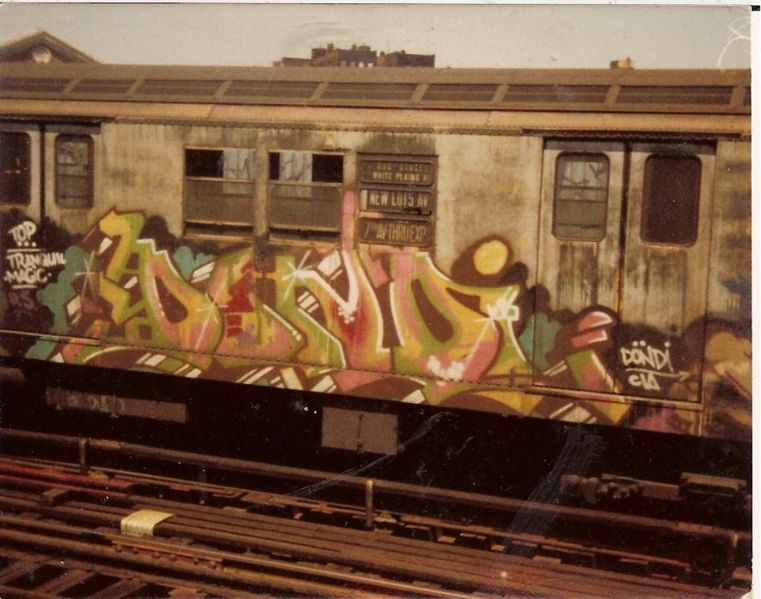
\includegraphics[width=0.8\textwidth]{Graphics/dondi}
	\caption[Fr�hes Graffiti-\emph{Piece} von \emph{Dondi},  \url{http://www.flickr.com/photos/sweet_child_of_mine/}]{Fr�hes \emph{Piece} auf New Yorker U-Bahn von \emph{Dondi}, 1979}
	\label{dondi}
\end{figure}
Im Verlauf der fr�hen 1970er Jahre schliessen sich die \emph{Writer}\footnote{zu deutsch: Schreiber, Akteure der Graffiti-Szene} zu \emph{Crews}\footnote{zu deutsch: Gruppe, Clique, auch Gang} zusammen, um dann gemeinsam Z�ge zu besprayen und sich vor drohenden Gefahren (Polizei, Hausbesitzer) zu warnen. 
\\%%
Ende der Siebziger schwappte das Ph�nomen auch nach Europa �ber, es bildeten sich Graffiti-Szenen in ganz Europa, auch in der Schweiz gab es einen regelrechten Graffiti-Boom.\footnote{\url{http://www.linguist.ch/graffitihistory.htm}, Autor unbekannt, Betrachtet:19.2.12}
\\%%
Mit dieser neuen Welle von Aufmerksamkeit weckte Graffiti pl�tzlich auch das Interesse des etablierten Kunstbetriebes. Es folgte eine Welle von Graffiti-Vernissagen und Ausstellungen, unter dem Label "`Street-Wear"' beeinflusste die Graffiti-Subkultur sogar Mode. In New York stellten auch bekannte Galerien wie Tom Shafrazi, Graffiti aus.
\\%%
Kommerzielle Graffiti in Galerien wurden zeitweise f�r Rekordpreise verkauft. Auch die mit Graffiti eng zusammenh�ngende Hip-Hop- und Breakdance-Kultur verschiebt sich in das Rampenlicht der Medien und erh�lt die Aufmerksamkeit der Massen. Jedoch im Gegensatz zu Hip-Hop ebbt der Boom um Graffiti in der Mitte der Achtziger wieder ab und nur wenige K�nstler k�nnen sich mit Graffiti ihren Lebensunterhalt verdienen. In Europa h�lt das Interesse l�nger an, flaute aber Anfang der Neunziger auch wieder ab.
\\%% 

\subsection{Gr�nde f�r die Nicht-Etablierung von Graffiti}
Oft wird bei der Etablierung der Graffitikunst in den 80ern Jean Michel Basquiat und Keith Haring als Beispiel angegeben und behauptet dass ja eigentlich eine Etablierung stattfand, da diese zwei K�nstler aus dem Graffiti-Umfeld sehr erfolgreich zu sein schienen. Sie waren jedoch keine echten Graffitik�nstler, sondern lediglich davon inspiriert.\footnote{\cite[S. 43]{austin2001}}\\
Den echten \emph{Writern} gelang die Etablierung im Kunstbetrieb nicht, sie scheiterten beim Eintritt in die Hochkultur aufgrund ihres fehlenden kunsthistorischen Wissens und ihrer sozialen Herkunft aus der unteren nordamerikanischen Gesellschaftsschicht.
\\%%
Die Frage, die sich nun stellt ist, ob es dem Ph�nomen Street-Art, das Mitte des letzten Jahrzents einen �hnlichen Aufmerksamkeitsschub erhalten hat, �hnlich ergehen wird, oder ob Street-Art wie \emph{Bustart}\footnote{Bustart ist ein Basler Street-Art-K�nstler, der momentan in Amsterdam seine Kunst vollzeitlich aus�bt. Interview im Anhang} sagt,  "`... eine neue Kunstepoche nach Popart"' ist. Um dem nachzugehen werde ich zuerst auf die Entwicklung von Street-Art eingehen.
\subsection{Entwicklung der Street Art}
Die Street Art entwickelte sich in den 80er Jahren aus der Graffitibewegung heraus. Viele Graffitik�nstler probierten neue Methoden aus, um sich im urbanen Raum auszudr�cken. Die Street-Artists waren auch meist deutlich �lter als der Altersdurchschnitt der \emph{Writer}, w�hrend diese meist um die 20 Jahre alt waren, waren Street-Artists meist f�nf bis zehn Jahre �lter und kannten sich gut mit der Graffiti-Szene aus und hatten teilweise auch ein gewisses Kunstverst�ndnis. Der Wechsel des Mediums von Freihand-Graffiti zu Schablonen, Sticker und Plakaten und Cut-Outs\footnote{Auf Papier gezeichnete oder gesprayte und dann ausgeschnittene und aufgeklebte Kunstwerke.} erschien ihnen logisch da der eigene Name auf einer Wand nur begrenzt Aussagekraft hatte und die Mittel der Street-Art vielseitiger und flexibler waren als nur die Spraydose.

%Es gab jedoch nach dieser fehlgeschlagenen Etablierung der Graffiti im Kunstfeld ein anderen Versuch der Graffiti-Szene, sich im etablierten Kunstfeld zu bew�hren.
%Obwohl Graffiti als Ganzes den Sprung in das etablierte Kunstfeld nicht schaffte, gibt es einige K�nstler, die sich mit Graffiti ihren Lebensunterhalt verdienen k�nnen und ihre Kunst in Galerien ausstellen und verkaufen. Diese K�nstler sind 





\section{Street-Art-Ans�tze und dessen Vertreter}
Ich werde nun die Entwicklung der Street-Art anhand einiger Pioniere beschreiben.
Bei Street-Art verschiebt sich die Intention der Arbeit. Street-Artist wollen nicht bloss ihren Namen m�glichst sch�n und h�ufig in der Stadt sehen sondern ihre Motivation ist um einiges facettenreicher. Es wird weniger auf Quantit�t und mehr auf Innovation, Kreativit�t und qualitative Umsetzung geachtet. Die Street-Art-K�nstler unterscheiden sich oft auch im Alter stark von den jungen Graffitisprayern.

\subsection{Blek le Rat und die Pochoiristen}
1981 fing der franz�sische Grafiker Xavier Prou unter dem Pseudonym \emph{Blek le Rat} an, die W�nde Paris' zu bespr�hen. Inspiriert durch die New-Yorker Graffiti-Szene, versuchte er ein amerikanisches Graffiti-\emph{Piece} zu malen. Dieser Versuch misslang jedoch und es wurde ihm klar, dass amerikanisches Graffiti nicht an Pariser W�nde passt. Er stieg auf die Schablonentechnik\footnote{Schablone heisst auf franz�sich Pochoir, daher der Name der Bewegung} um und begr�ndete somit im Prinzip die Schablonenkunst. \footnote{\cite[S. 42]{reinecke2007}}%\footnote{Julia Reinecke, \emph{Street-Art - Subkultur zwischen Kunst und Kommerz}, 2007, S. 42}
\\
\begin{figure}[h!]
	\centering
	\subfloat[Tom Waits, 1983]{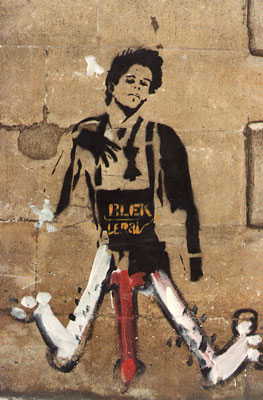
\includegraphics[width=0.3\textwidth]{Graphics/blek1}}
	~
	\subfloat[Schreiender Mann, 1984]{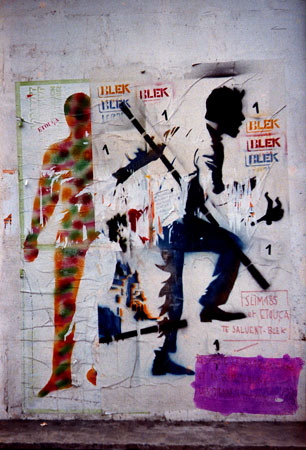
\includegraphics[width=0.3\textwidth]{Graphics/blek2}}
	~
	\subfloat[Selbstportrait, 1986]{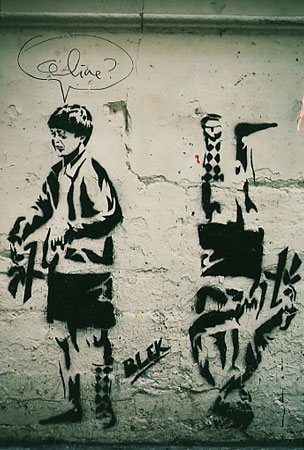
\includegraphics[width=0.3\textwidth]{Graphics/blek3}}
	\caption[\emph{Ble le Rats} Portraits in den 1980ern, \url{http://bleklerat.free.fr/stencil\%20graffiti.html}]{\emph{Ble le Rats} Portraits in den 1980ern}
\end{figure}

Schablonen verbreiteten sich in Frankreich sehr rasch, da sie im Voraus angefertigt werden konnten und dann beim eigentlichen spr�hen weniger Geschick und dadurch Zeit ben�tigt wird. Diese Technik breitete sich dadurch sehr rasch aus und viele K�nstler wandten sich vom \emph{Writing} ab, um ihre Spuren nun mit Schablonen an den W�nden zu hinterlassen.
\\%%
Prous Motive reichen von Ratten zu Pflanzen und Ganzk�rper-Portraits von bekannten K�nstlern und Musikern wie z.B Tom Waits oder Andy Warhol. Im Gegensatz zur rebellischen Nachricht, die viele Graffitisprayer durch ihre \emph{Tags} an die �ffentlichkeit richten, will Prou mit seinen Schablonenwerken eher die Umwelt und Gesellschaft reflektieren.
"`I am more interested in showing the world that urban art is more than just art of rebellion, but an artform that speaks about poetry and everyday life and is a reflection of our society"'\footnote{Reinecke, 2007, S. 54}
\\%%
Die Pochoir-Bewegung, also die franz�sische Schablonenkunst-Szene, vermischte sich in den 90ern mit anderen Street-Art-Bewegungen und der Gebrauch von Schablonen verbreitete sich rasch auf der ganzen Welt und wurde zu einer der Haupttechniken der Street-Art.
\\%%
Blek le Rat verringerte seine Aktivit�t um das Jahr 1991 aus famili�ren Gr�nden, begann jedoch Ende der 90er wieder aktiver zu werden und ist heute einer der  am l�ngsten aktiven Street-Artists.

\subsection{Shepard Fairey: Propaganda f�r Nichts}
1989 begann Shepard Fairey, Student an der RISD\footnote{Rhode Island School of Design}, mit der bis heute weltweit gr�ssten Propagandakampagne, jedoch ohne etwas propagieren oder eine Aussage verbreiten zu wollen, sondern einzig mit dem Graffitiziel des \emph{Getting-Up}\footnote{\emph{Getting-Up} bezeichnet im Graffitijargon das Hinausgehen und seinen Namen in der Stadt zu verteilen.}. Seine \emph{Obey-Giant}\footnote{\emph{to obey}, zu deutsch: jemandem gehorchen, einem Befehl Folge leisten.}-Aufkleber, -Poster und -Schablonenbilder sind fast �berall auf der Welt zu finden, und fast jeder amerikanische Stadtbewohner hat schon einmal eines von Shepards Werken gesehen. Hinter dieser Kampagne steckt keine Botschaft, die Aufkleber und Poster sind nach Fairey an sich bedeutungslos, sie erhalten ihre Kraft erst durch die Reaktion der Menschen auf diese 
scheinbar sinnlosen Plakate.
\\%%
\begin{figure}[h!]
	\centering
	\subfloat[Obey-Sticker]{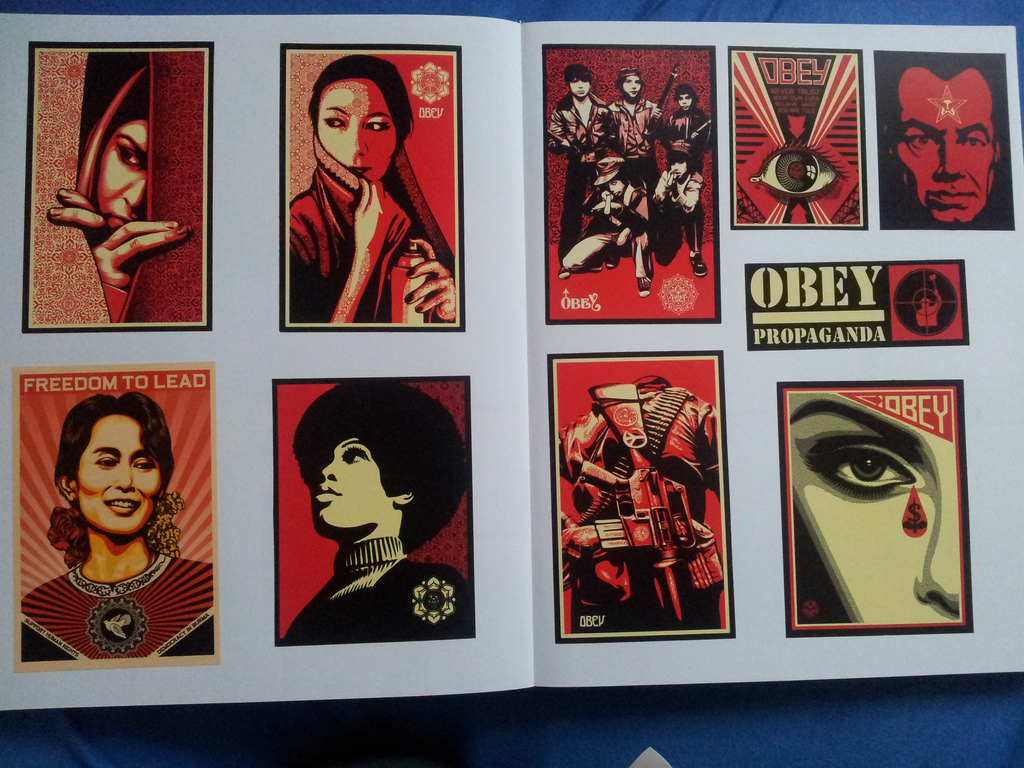
\includegraphics[width=0.5\textwidth]{Graphics/obey}}
	~
	\subfloat[Stilisiertes Andr�-the-Giant-Plakat in New York]{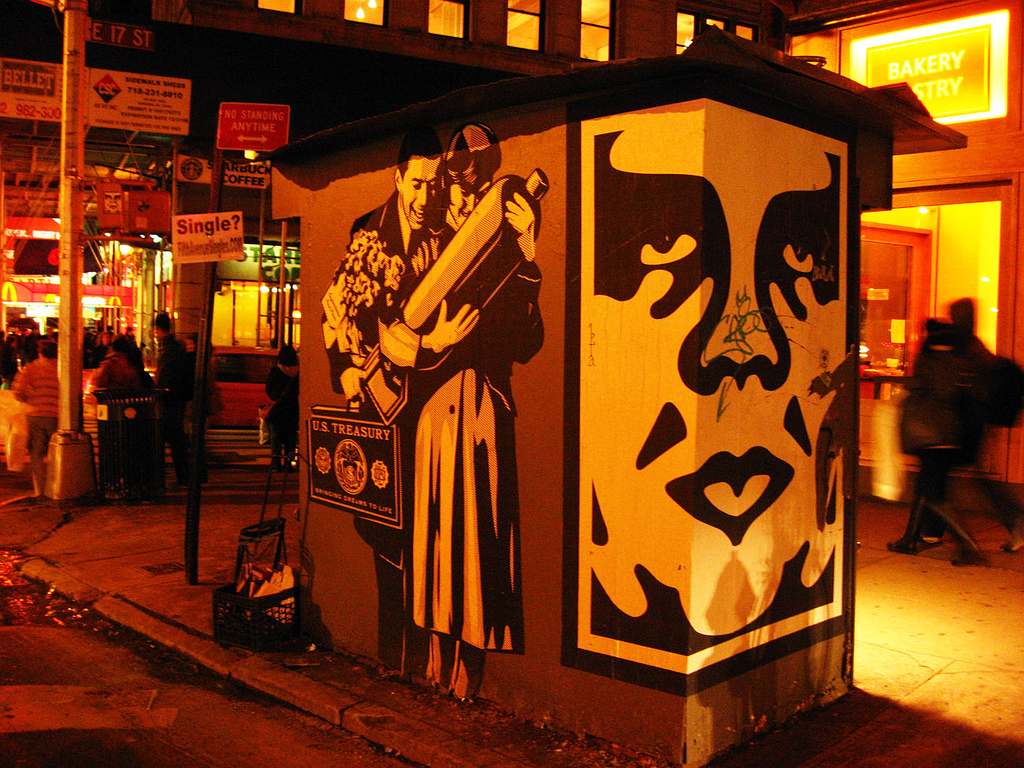
\includegraphics[width=0.5\textwidth]{Graphics/obey3}}
	\caption[Shepard Fairey's Plakate und Sticker]{Shepards Ausbildung als Grafikdesigner spiegelt sich in seinen Werken wider.}
\end{figure}

Die Motive, die sich zum Grossteil um die Figur \emph{Andr� the Giant}\footnote{Andr� Ren� Roussimoff, bekannt unter \emph{Andr� the Giant}, war ein franz�sischer Professioneller Wrestler und Schauspieler.} drehen, sind sehr einpr�gsam und der kurze Slogan oder das Stichwort darunter so eing�ngig dass die Aufkleber einer Werbekampagne �hneln. Shepard will die �ffentlichkeit provozieren und sie zum kritischen hinterfragen anregen indem er Werbung f�r etwas macht, was gar nicht existiert.\footnote{Reinecke, 2007, S. 48}
\\%%
Fairey nutzt die Strasse als Medium, wo er frei walten kann und nicht an Zensur oder Regeln gebunden ist.
\\%%
Doch anders als andere Street-Artists stammt Fairey nicht aus der Graffiti-Szene, sondern wurde haupts�chlich vom Skateboardfahren und von der Punkrockmusik inspiriert. \footnote{Wikipedia Artikel �ber Shepard Fairey, \url{http://en.wikipedia.org/wiki/Shepard_Fairey}, Angeschaut: 19.2.12}
\\%%
Fairey verkauft Drucke und Aufkleber und auch T-Shirts und andere Kleidungsst�cke. Die von ihm lizenzierte Bekleidungsfirma \emph{Obey Giant Clothing} designt und verkauft Pullover, Hosen, Jacken und andere Kleidungsst�cke. Er ist somit eigentlich eher Designer als K�nstler, stellt seine Werke jedoch auch in Galerien und Ausstellungen aus.\footnote{Lindsay William-Ross, \url{http://laist.com/2008/04/07/shepard_fairey_blek_le_rat_subliminal_projects.php}, Betrachtet am 19.2.12}
\\%%
Fairey lebt mittlerweile vom Verkauf von Kleidern und Drucken sowie Originalen seiner Arbeit. Er ist nicht mehr sehr aktiv auf der Strasse und klebt nicht mehr viele Poster auf. Deshalb wird er von vielen Street-Artists als \emph{Sell-Out}\footnote{Jemand der sich dem Kommerzialismus hingegeben hat und keine eigentliche, illegale Street-Art auf der Strasse mehr macht} bezeichnet. 

\subsection{Banksys provokative Schablonengraffiti}
\begin{figure}[h!]
	\centering
	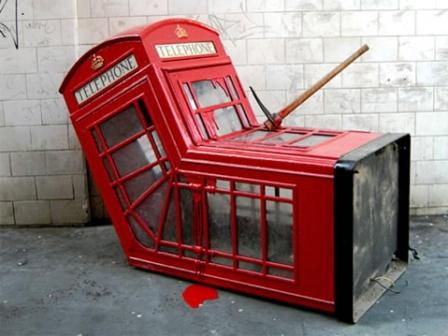
\includegraphics[width=1\textwidth]{Graphics/banksy_london}
	\caption[Banksys deformierte Telefonkabine in London, 2008]{Banksys deformierte Telefonkabine in London, 2008}
\end{figure}
Banksy ist mit Abstand der bekannteste Street-Art-K�nstler und stellte seine Werke schon in vielen Galerien und Ausstellungen aus. Im Gegensatz zu Shepard Fairey ist Banksy jedoch trotz seines grossen Erfolgs immer noch auf der Strasse t�tig und reist um die Welt um seine Werke international anzubringen.
\\%%

Sein Erfolg erm�glicht ihm jedoch auch aufw�ndigere Werke, zum Beispiel eine eigene Bronzestatue, die er in einem Park platzierte, oder eine modifizierte alte Londoner Telefonkabine. Seine meist schwarz-weissen Schablonenkunstwerke prangern oft politische Misst�nde an oder richten sich gegen exzessive  �ffentliche Werbung. Er kritisiert jedoch nicht banal und direkt, sondern ironisch und satirisch. Er regt zum Denken an und zw�ngt dem Betrachter nicht plump eine politische Parole auf, was gute Street Art laut Hans-Christian Psaar unter anderem ausmacht.\footnote{psaar2007}
\\%% 
An seine Ausstellungen kommen auch Prominente wie z.B Angelina Jolie und Brad Pitt sowie bekannte Kunstkritiker. Banksy ist einer der wenigen Street-Art-K�nstler die sich im etablierten Kunstfeld bew�hrt haben ohne dabei an \emph{Street Credibility}\footnote{Im Graffitijargon die Anerkennung von anderen Graffiti-K�nstlern} zu verlieren. So erzielten seine Werke �usserst hohe Preise beim britischen Auktionhaus Sotheby's.\footnote{\cite{sothebys2010}}
\begin{figure}[h!]
	\centering
	\subfloat{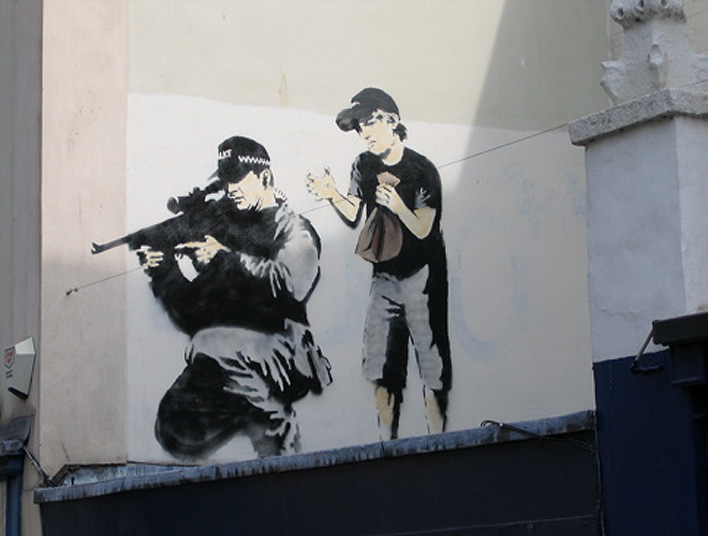
\includegraphics[width=0.3\textwidth]{Graphics/banksy1}}
	~
	\subfloat{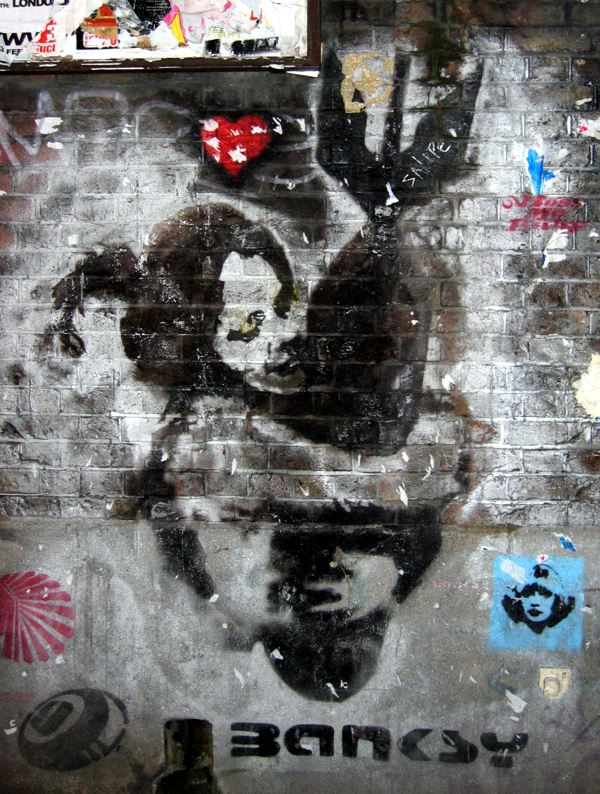
\includegraphics[width=0.3\textwidth]{Graphics/banksy2}}
	~
	\subfloat{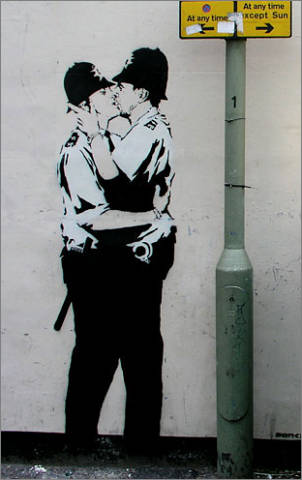
\includegraphics[width=0.3\textwidth]{Graphics/banksy3}}
	\caption[Banksys Street-Art in London, \url{http://www.holytaco.com/25-coolest-banksy-graffiti/}]{Banksys Street-Art in London}
\end{figure}

\subsubsection{Exit Through the Gift Shop}

2010 ver�ffentlichte Banksy \emph{Exit Through the Gift Shop}, ein als Dokumentarfilm aufgemachter Film, oder, wie Banksy sagt eine "`Mockumentary"'\footnote{Ein Kofferwort das sich aus dem englischen, \emph{to mock}: verspotten, sich �ber etw. lustig machen, und \emph{documentary}: Dokumentarfilm, zusammensetzt}, also ein Dokumentarfilm der eigentlich gar keiner ist. \\
Im Film geht es um den Hobby-Filmer Thierry Guetta, der durch Zufall mit der Street-Art-Bewegung in Kontakt kommt und Street-Art-K�nstler auf der ganzen Welt mit der Kamera verfolgt, um daraus einen Dokumentarfilm zu machen. Daran scheitert Guetta jedoch und Banksy hilft ihm, indem er den Spiess umdreht und die Kamera auf Guetta richtet. Guetta wird nun selbst aktiv und beginnt auf Rat Banksys selbst Kunst zu machen. Er f�ngt gleich gross an, verkauft all sein Hab und Gut und finanziert sein Haus neu um sich eine Siebdruckanlage, eine vollst�ndige K�nstlercrew sowie eine leerstehende Lagerhalle zu kaufen und beginnt "`Kunst"' zu machen. Er selbst schwingt jedoch nicht den Pinsel, sonder beauftragt seine Angestellten, die Kunstwerke nach seinen Ideen anzufertigen. Die Ausstellung "`seiner"' Werke wird ein totaler Erfolg, die Leute sind begeistert, und Guetta verkauft Kunst im Wert von knapp einer Million US-Dollar.\\
Banksy will mit dem Film den kommerziellen Kunstmarkt satirisch beleuchten, indem er zeigt dass es f�r eine Etablierung im kommerziellen Kunstmarkt eigentlich gar keine k�nstlerischen F�higkeiten braucht. \emph{Exit Through the Gift Shop} ist satirisch und beleuchtet ironisch die kommerzielle Kunstwelt, sowie die Verbogenheit des Kunstmarktes. Er zeigt dass jemand der �berhaupt keinen k�nstlerischen Hintergrund und kaum Talent hat, es trotzdem schaffen kann eine Ausstellung auf die Beine zu stellen und Kunstwerke teuer zu verkaufen.
\\%%
Banksy selbst sagt �ber den Film folgendes: 
\begin{quote}
\emph{"`I guess my ambition was to make a film that would do for graffiti art what �The Karate Kid� did for martial arts � a film that would get every schoolkid in the world picking up a spray can and having a go�As it turns out, I think we might have a film that does for street art what �Jaws� did for waterskiing."'}\\(\cite{jones2010})
\end{quote}
Dies verdeutlicht, dass Banksy eigentlich bis zur H�lfte des Films gar nicht wusste, dass es ein Film wird, und dass der Film drehbuchlos, chaotisch und unorganisiert daherkommt, was aber nicht negativ zu werten ist, sondern nach Filmkritikern die Street-Art-Bewegung widerspiegelt und zum Film passt.\footnote{\cite{baumgardt2010}}


\subsection{Street Art in der Schweiz}
In der Schweiz gab es in den 1980er-Jahren einen grossen Graffitiboom. Basel ist heute noch eine bedeutende Graffiti-Stadt. Einige K�nstler stiegen von Graffiti auf Street-Art um und so gibt es auch eine kleine Street-Art-Szene in der Schweiz. Ich interviewte zwei Basler Street-Art-K�nstler: Zum einen den jetzt in Amsterdam lebenden Bustart, sowie Seifrei, der vor allem durch seine Paste-Ups\footnote{Mit Kleister an die Wand geklebte Plakate} eines Roboters in der Stadt auff�llt. Beide hatten ihre Wurzeln in der Graffiti-Bewegung und beide wurden stark von Banksy inspiriert. Beide k�nnen oder konnten in der Schweiz nie von ihrer Kunst leben, weil das einerseits nicht ihr Ziel ist/war und andererseits weil daf�r in der Schweiz praktisch kein Markt existiert und nur wenig Street-Art Ausstellungen stattfinden.\\
Laut Seifrei ist der internationale Street-Art-Boom verursacht durch Banksy nur eine Phase und wir �hnlich wie der Graffiti-Boom in den 1980ern langsam wieder abflauen. Er ist hauptberuflich Lehrer und hat auch nicht vor von seiner Street-Art zu leben, im Gegensatz zu Bustart, der nach Amsterdam gezogen ist um dort mit seiner Kunst ein gr�sseres Publikum erreichen zu k�nnen und um dann vielleicht den Sprung ins etablierte Kunstfeld zu schaffen. \\
Die vollst�ndigen Interviews mit den beiden Street-Art-K�nstlern sind im Anhang zu finden.
\begin{figure}[h!]
	\centering
	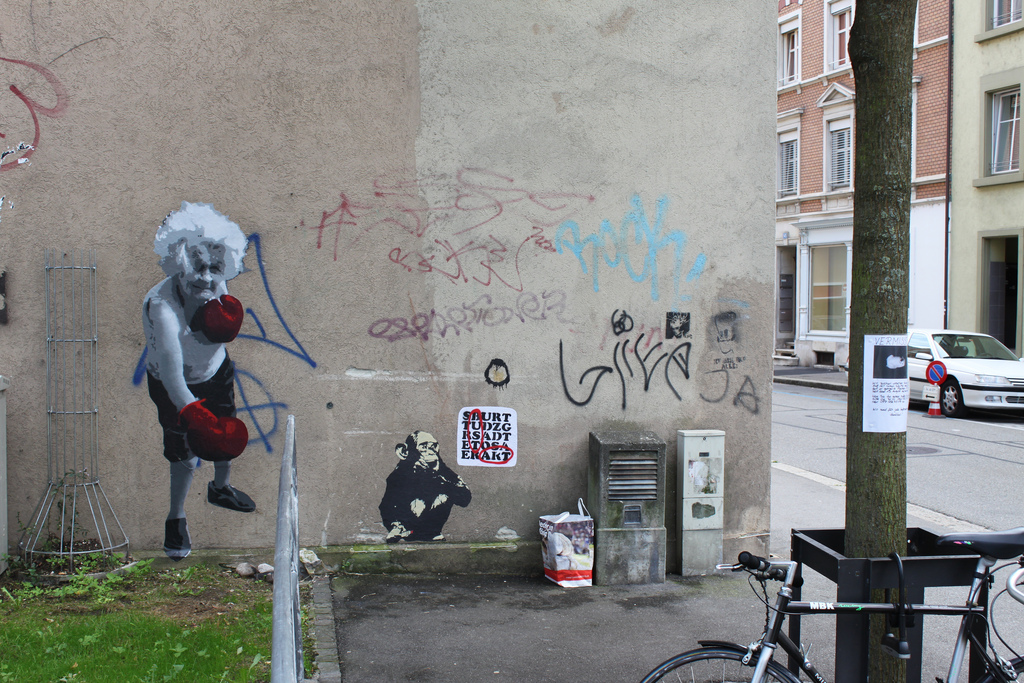
\includegraphics[width=1\textwidth]{Graphics/bust_seifrei}
	\caption[Bustart und Seifrei in Basel, \url{http://www.flickr.com/photos/befreee/4932425184/sizes/l/in/photostream/}]{Seifrei (links) und Bustart (rechts) in Basel}
\end{figure}
%************************************************
\chapter{Street-Art als angewandte Kunst}
\label{chp:kapitel2}
%************************************************

\section{Bildende und angewandte Kunst}
Die Kunst kann man grob in zwei Bereiche unterteilen: Bildende und angewandte Kunst. Die bildende Kunst, franz�sisch \emph{les Beaux-Arts}, also die sch�nen K�nste, definiert sich im engeren Sinne durch den etablierten Kunstmarkt und -betrieb, zu dem Vetreter der Kunstkritik, Kunsth�ndler sowie Sammler und Kunstmuseen geh�ren.\\
Sie grenzt sich von der darstellenden Kunst, wie Theater und Film, sowie der Literatur und Musik ab.
\\%%
Als Angewandte Kunst, auch Kunstgewerbe genannt, bezeichnet man die handwerkliche oder maschinelle Herstellung von Gebrauchsgegenst�nden mit k�nstlerischem Anspruch.
Street Art f�llt nun nicht direkt unter diese Definition, doch wenn man die N�he zur Werbung betrachtet wird dies klarer.
\subsection{Werbung als angewandte Kunst}
Werbung wurde schon Anfang des 19. Jahrhunderts von der bildenden, damals freien, Kunst getrennt. K�nstler die Werbung gestalteten wurden von den "`freien"' K�nstlern weniger gesch�tzt als andere "`freie"' K�nstler. Also schon damals wurde Werbung vom Rest der Kunstwelt abgetrennt. Seither hat sich das kaum ge�ndert. Die K�nstler der Werbeindustrie sind oft Grafikdesigner und Fotografen und werden dem Kunsthandwerk, also der angewandten Kunst angerechnet. Auch mehrere Versuche der Werbebranche in den 1980ern und 1990ern, sich der bildenden Kunst gleichzustellen, verliefen erfolglos.\footnote{\cite[S. 144]{reinecke2007}}. Michael Schirners provokative Aussage "`Werbung ist Kunst"'\footnote{\cite{turner1988}} warf zwar einige heisse Diskussionen auf, verhalf aber schlussendlich der Werbung nicht, in die "`Sch�nen K�nste"' eintreten zu k�nnen. Dies lag unter anderem daran, dass er einer der wenigen Stimmen der Werbung im etablierten Kunstbetrieb war.\footnote{\cite[S. 145]{reinecke2007}}

\subsection{Street Art und dessen N�he zu Werbung}
Street Art teilt gen�gend Elemente mit Werbung um sie als angewandte Kunst bezeichnen zu k�nnen. Dies werde ich im Folgenden erl�utern.\\
Werbung und Street-Art zielen beide auf dieselbe Zielgruppe ab, n�mlich auf alle Personen. Sie beanspruchen beide denselben Raum und k�mpfen auch darum. Der Street-Art-K�nster \emph{publicadcampaign} verwandelt durch das Ersetzen von Werbeplakaten in Schauk�sten diese in Street-Art-Kunstwerke.\\
\begin{figure}[h!]
	\centering
	\subfloat{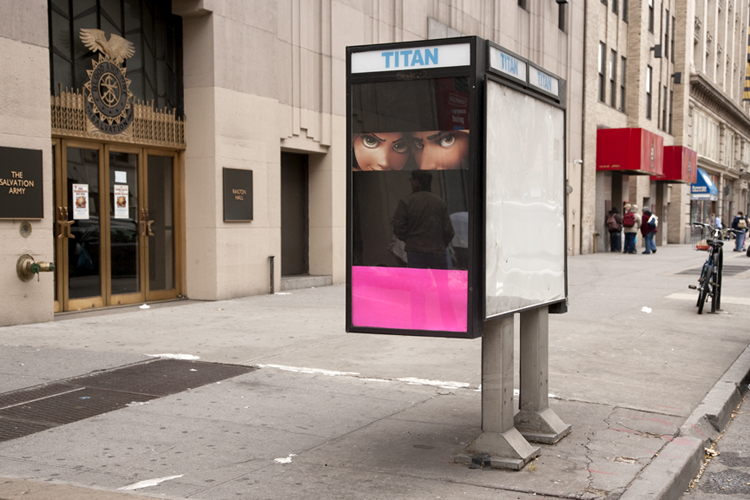
\includegraphics[width=0.5\textwidth]{Graphics/public1}}
	~
	\subfloat{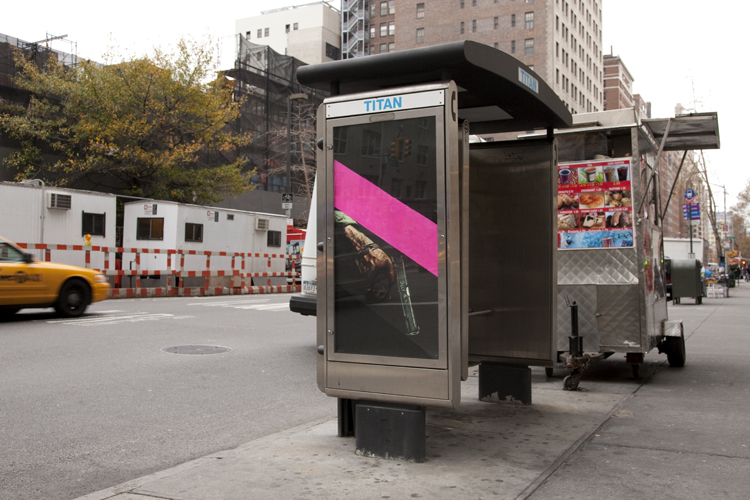
\includegraphics[width=0.5\textwidth]{Graphics/public2}}
	\caption[Mit Tempera ver�nderte Werbeschauk�sten von \emph{publicadcampaign}, 2010, \url{http://www.publicadcampaign.com/ongoing/let-me-handle-this/}]{Mit Tempera ver�nderte Werbeschauk�sten von \emph{publicadcampaign}, 2010}
\end{figure}
Werbung und Street-Art k�mpfen also beide um die Aufmerksamkeit der Leute und sie tun es oft auch auf dieselbe Art und Weise. Street-Art-K�nstler verwenden meist die gleichen Grafikdesignprogramme, um ihre einpr�gsamen und ikonischen Charaktere herzustellen. Werbung und Street-Art bedienen sich beide h�ufig des \emph{Character Designs}, also der Gestaltung von m�glichst wiedererkennbaren Figuren, die dann wie das Logo einer Firma, das Markenzeichen eines Street-Artists ist.\\
%%Bild sticker, werbeplakat
Viele Street-Art-K�nstler vervielf�ltigen ihre Poster und Aufkleber auch industriell, gleich wie Werbefirmen. Die Werbeindustrie sch�pft auch aus der Street-Art. So stammmt die Stickerkunst urspr�nglich aus der Street-Art-Szene. Mittlerweile gibt es viele Firmen, die an ihre Kunden Sticker verteilen damit diese f�r ihre Waren werben.
Doch Street-Art kann man nicht nur durch ihre N�he zur Werbung zur angewandten Kunst z�hlen es ist auch der sogenannte Habitus der Street-Art entscheidend.
\section{Kapitalformen in der Street Art}
\subsection{Kapitalformen nach Bourdieu}
Der franz�sische Soziologe Pierre Bourdieu unterteilte bei seinen Verhaltensstudien in der franz�sischen Gesellschaft das Kapital in verschiedene Formen. F�r ihn war das Kapital nach wirtschaftlicher Definition nur eine Form des Kapitals, n�mlich das �konomische Kapital, was sich ausschliesslich aus materiellem Reichtum zusammensetzt. �konomisches Kapital muss nicht unbedingt Geld sein, aber es darf keinen kulturellen oder symbolischen Wert haben. Das meiste Eigentum ist �konomisches Kapital.
\subsubsection{Kulturelles Kapital}
Die zweite Form des Kapitals ist nach Bourdieu das kulturelle Kapital. Dieses wird in drei Teilformen unterteilt: Beim objektivierten Kulturkapital ist das Kapital an ein Objekt gebunden. Objektgebundenes Kapital liegt meist in Form von B�chern, Musik-CDs oder eben Kunstwerken vor. Dieses Kapital kann relativ rasch durch Verkauf in �konomisches Kapital umgewandelt werden. Schwieriger ist dies beim inkorporierten und institutionalisierten Kapital. Das inkorporierte Kapital ist die personengebundene Kultur, die sich eine Person im Verlaufe ihres Lebens aneignet. Mit dem personengebundenen Kapital sind s�mtliche erlernbare F�higkeiten gemeint, die einer Person durch Erziehung der Eltern in ihrer Kindheit beigebracht wurden, oder die eine Person sich selbst angeeignet hat. Der Wert dieses Kapitals setzt sich aus der Zeit zusammen, die daf�r investiert wurde. Wird die Ausbildung an einer Hochschule mit einem Abschluss beendet, liegt ein institutionalisiertes Kapital vor. \\Kulturelles Kapital kann dar�berhinaus in zwei andere Formen unterteilt werden. Schliesst man mit einem Titel eine Universit�t ab, besitzt man legitimes kulturelles Kapital. Autodidakten, also Leute die sich Wissen selbst beibringen, verf�gen, auch wenn sie in ihren kulturellen Kompetenzen den Titeltr�gern �berlegen sind, lediglich �ber sogenanntes illegitimes Kulturkapital. Meistens entscheidet jedoch das legitime institutionelle Kapital �ber das Einkommen, und damit �ber den materiellen Wert des Kapitals.\footnote{Wikipedia, betrachtet am 19.2.12, \url{http://de.wikipedia.org/wiki/Kapital}}
\subsubsection{Soziales Kapital}
Als dritte Form des Kapitals bezeichnet Bourdieu das soziale Kapital. Es besteht aus den sozialen Verbindungen innerhalb einer Gruppe. Verf�gt ein K�nstler zum Beispiel �ber hohes soziales Kapital, kann er immer mit der Unterst�tzung in der Street-Art-Bewegung, seiner Gruppe, rechnen. Das soziale Kapital basiert auf gegenseitigem Kennen und Anerkennen sowie der Zugeh�rigkeit zu einer bestimmten Gruppe.
\subsubsection{Symbolisches Kapital}
Das Kapital, das zuerst von aussen wahrgenommen wird, ist das symbolische Kapital. Es ist die gesellschaftliche Anerkennung und Wertsch�tzung gegen Aussen. Es tritt meist mit den anderen Kapitalformen auf und verst�rkt die Wirkung dieser. Das symbolische Kapital ist auch unter Prestige oder Renommee bekannt.\footnote{\cite[S. 128-129]{reinecke2007}}
\subsection{Anwendung der Kapitalformen auf die Street Art}
In der Street-Art-Bewegung ist das soziale Kapital das wichtigste, da durch die Anonymit�t der K�nstler die Kommunikation haupts�chlich innerhalb der Street-Art-Szene stattfindet, und, ausser durch sporadische Zeitungsartikel, die K�nstler kaum mit der �ffentlichkeit in Kontakt treten. Das Netzwerk eines Street-Artists vergr�ssert sich deshalb ausschliesslich durch pers�nliche Kontakte.
\\
F�r den Eintritt in die Welt der bildenden Kunst ist meistens - durch ungesagte, von renommierten Kunstkritikern und Kuratoren verordneten Regeln - ein hohes legitimes institutionalisiertes Kapital erforderlich. Einem K�nstler mit Abschluss an einer Kunsthochschule f�llt es, egal wie hoch sein inkorporiertes kulturelles Kapital auch ist, \emph{viel} leichter sich im etablierten Kunstfeld zu bew�hren als zum Beispiel den brasilianischen Zwillingsbr�der Os G�meos, deren Ausbildung "`die Strasse"' war.\footnote{\cite{derwanz2010}} Im Bereich der Street-Art haben die K�nstler meist kein institutionelles Kulturkapital, da nur wenige eine Kunsthochschule besucht haben und da die Kunstform urspr�nglich nicht aus anderen Kunstformen, sondern aus einer Subkultur hervorgegangen ist. \\
Deshalb wird, egal wie gut die Werke des einzelnen K�nstlers sind, Street-Art auch nicht von der etablierten Kunstwelt als "`sch�ne Kunst"' bezeichnet sondern der Trivialkultur, und damit der angewandten Kunst, zugeordnet. Wenn ein Street-Art-K�nstler nun den Schritt in die Hochkultur schaffen will, muss er ein hohes symbolisches und soziales Kapital besitzen, um sich (durch Anerkennung und Unterst�tzung durch die Street-Art-Szene) bei Galeristen und Kuratoren behaupten zu k�nnen. 

\section{Gemeinsamkeiten von Street Art und bildender Kunst}
Obwohl Street-Art, wie eben erl�utert, zu den angewandten K�nsten z�hlt, kann eine gewisse Verbindung zu bildenden Kunstformen hergestellt werden.
\subsection{Dada}
Dada war eine k�nstlerische und literarische Bewegung Anfang des 19. Jahrhunderts, die sich durch die Parodisierung und Ablehnung konventioneller Kunst auszeichnete. Sie war im Prinzip eine Auflehnung gegen die traditionelle Kunst der K�nstler selbst.\footnote{Wikipedia, betrachtet am 19.2.12, \url{http://de.wikipedia.org/wiki/Dada}}
Marcel Duchamp war einer der Hauptakteure der Dada-Bewegung und erregte mit seinen \emph{Ready-Mades}, auf die ich in Kapitel 4.1 noch kurz eingehen werden, grosses Aufsehen. Ready-Mades waren einfache Gebrauchsgegenst�nde, die Duchamp ohne Qualit�tskriterien aussuchte, und dann mit einem Synonym signierte. Durch den neuen Kontext in den der Gegenstand gesetzt wurde, wurde er zum wertvollen Kunstwerk\\
Die Street-Art verwendet einige Techniken, die es schon im Dada gab. Zum einen wurden im Dada teilweise schon Schablonen verwendet, zum Beispiel von Kurt Schwitters oder John Hartfield\footnote{\cite[S. 153]{reinecke2007}}. Auch die Verwendung von Plakaten ist eine Gemeinsamkeit der beiden Kunstformen. Mit dieser Form wenden sich beide Kunstformes direkt an die �ffentlichkeit, was aber bei Street-Art immer der Fall ist. Die Dada-Kunst hat keine bestimmten Merkmale, sie versteht sich eher als Anti-Kunst die die bestehenden Kunstformen in Frage stellte. Auch verschiedene Street-Art-K�nstler lehnen das Kunstfeld und dessen Regeln und Prestige ab und versuchen durch die Platzierung ihrer Arbeiten im �ffentlichen Raum die T�rsteher-Funktion der etablierten Galerien und Museen zu umgehen. Der Aktivismus gegen die tradionelle Kunst ist eine wichtige Gemeinsamkeit von Dadaismus und Street-Art.
\\

\subsection{Situationismus}
1957 wurde in Italien die linksradikal orientierte Situationistische Internationale, kurz, S.I., gegr�ndet. Obwohl die Organisation in Italien gegr�ndet wurde, agierte sie international und die Zahl ihrer Mitglieder schwankte zwischen zehn und �ber 40.\\
Zwei Techniken der situationistischen Bewegungung lassen sich besonders mit der Street-Art-Bewegung in Verbindung setzen: Das \emph{d�rive}\footnote{Auf Deutsch: umherschweifen} und das \emph{d�tournement}\footnote{Auf Deutsch: Zweckentfremdung}.\\
Beim \emph{d�rive} treffen sich die Situationisten an einem Punkt in der Stadt und schweifen dann von diesem Punkt in alle Richtungen aus, um die Stadt neu zu entdecken. Dies �hnelt stark dem sogenannten \emph{urban exploring}, dem st�dtischen Erkunden, welches in der Street-Art sehr wichtig ist, um neue Wege zu finden, den urbanen Raum f�r sich zu beanspruchen.\\
\begin{figure}[hb!]
	\centering
  
\includegraphics[width=0.7\textwidth]{Graphics/blf}
	\caption[Mc Donalds Kritik der \emph{Billboard Liberation Front}, \url{http://laughingsquid.com/billboard-liberation-front-to-serve-man/}]{Mc Donalds Kritik der \emph{Billboard Liberation Front} zum 50-J�hrigen Geburtstag des Fast-Food-Riesen}
\end{figure}
Das \emph{d�tournement} ist eine Technik, bei der vorhandene Werbeplakate leicht ver�ndert werden, sodass die Marke erkennbar bleibt, die Absicht und Botschaft des Plakates jedoch negiert oder sogar umgekehrt wird.\footnote{\cite[S. 155]{reinecke2007}}. Diese Technik hat Gemeinsamkeiten mit den modernen \emph{Adbusters}\footnote{Auf Deutsch: die Werbe-Sprenger} oder der \emph{Billboard Liberation Front}\footnote{Auf Deutsch: Reklametafel-Befreiungsfront}, einer Street-Art-Gruppe, die es sich zum Ziel gemacht hat, weltweit die Aussage von Werbetafeln zu entfremden und umzukehren.





%************************************************
\chapter{Etablierung von Street-Art}
\label{chp:kapitel3}
%************************************************

Im folgenden Kapitel werde ich auf den Kunstmarkt und den Bezug der Street-Art dazu eingehen sowie erl�utern warum sich Street-Art besser eignet in den etablierten Kunstmarkt
einzutreten als Graffiti.

\section{Was macht den Wert eines Kunstwerkes aus?}
Meiner Meinung nach ist Kunst dann Kunst, wenn der K�nstler sowie der Betrachter es als Kunst bezeichnet und jemand bereit ist, daf�r Geld zu zahlen. Doch wie wird bestimmt, wieviel ein bestimmtes Kunstwerk wert ist? Aus was setzt sich der Wert eines Kunstwerkes auf dem Kunstmarkt zusammen?
\\%%
Normalerweise wird der Wert eines Kunstwerkes durch Angebot und Nachfrage bestimmt. So viel, wie jemand bereit ist f�r ein bestimmtes Werk zu zahlen, so hoch ist der Marktwert eines Kunstwerkes. Doch es l�sst sich auch theoretisch ein Marktwert ermitteln. Dieser setzt sich aus zwei Dinge zusammen: Einerseits aus der handwerklichen Qualit�t des Werkes, wie dem Duktus des Gem�ldes oder der Verarbeitung der Statue. Andererseits, und dieser Punkt wird meist viel schwerer gewichtet, setzt sich der Wert eines Kunstwerkes aus dessen Symbolwert zusammen. Mit Symbolwert ist die etwas schwer greifbare symbolische Aufladung eines Werkes gemeint, die zur materiellen Wertsteigerung eines Werkes beitr�gt.
\\
Den tats�chlichen Marktwert durch Angebot und Nachfrage zu bestimmen ist bei Street-Art leider etwas schwierig bei, da die meisten Street-Art-Kunstwerke gar nicht zum Verkauf stehen und man viele K�ufe analysieren m�sste um eine Aussage �ber die ganze Street-Art-Szene machen zu k�nnen. Darum versuche ich, durch eine Ann�herung an  den Symbolwert, eine hypothethische Aussage �ber das momentane Potential der Street-Art auf dem Kunstmarkt zu treffen.\\
Isabelle Graw hat in ihrem Buch \emph{Der grosse Preis: Kunst zwischen Markt und Celebrity-Kultur} die Bestimmung des Symbolwerts in sieben Kriterien unterteilt, welche erf�llt werden m�ssen, wenn ein Kunstwerk symbolischen Wert haben soll: \emph{Singularit�t, kunsthistorische Zuschreibung, Etabliertheit des K�nstlers, Originalit�tsverheissung, Versprechen auf Dauer, Autonomiepostulat und intellektueller Anspruch.}
Ein Beispiel, wie stark der Wert eines Kunstwerkes vom Symbolwert abh�ngt, sind Marcel Duchamps \emph{Readymades}, die im ersten Viertel des letzten Jahrhunderts viel Aufmerksamkeit erregten. Dies sind normale Gebrauchsgegenst�nde, ein Flaschentrockner zum Beispiel, die nur durch die Signatur, im Falle des Flaschentrockners nicht einmal die von Duchamp selbst sondern die seines Pseudonyms, zu wertvollen Kunstwerken wurden. Der Wert setzte sich also nur aus dem Symbolwert zusammen.
\\%%
Ich habe diese sieben Kriterien nun auf die Street-Art angewandt um zu er�rtern, inwiefern die Street-Art als ganzes nun einen solchen Symbolwert besitzen kann. Schlussendlich kommt es jedoch auf die einzelnen K�nstler und Kunstwerke an, ob ein Werk einen Symbolwert besitzt oder nicht.

\section{Der Symbolwert von Street-Art-Kunstwerken}

\subsection{Singularit�t}
Street-Art ist eine in-situ-Kunstform, das heisst, jedes Werk wird durch die Installation an einem bestimmten Ort zu einer bestimmten Zeit einzigartig. Dies geht jedoch teilweise bei der �bertragung in die Galerie verloren, da dort der Ort und die Zeit keine Rolle mehr spielt. Manchmal wird der Street-Art sogar auf der Strasse diese Eigenschaft entzogen indem das St�ck Wand, auf dem sich das Werk befindet, abgetragen und dann verkauft wird.\footnote{Zum Beispiel bei einem Banksy-Werk in Jamaica. Zu sehen hier: \url{https://vimeo.com/2309114}}
\\
Rik Reinking\footnote{Kunstsammler, -h�ndler, Kurator und Veranstalter von Street-Art-Ausstellungen, auf ihn wird im Kapitel \emph{Ausstellungen und Galerien} genauer eingegangen} differenzierte in seiner Ausstellung \emph{Fresh air smells funny} zwischen sogenannten "`donated-to-the-streets"'-Arbeiten, also solchen die f�r die Strasse gedacht sind, und Werken, die f�r den Innenraum angefertigt wurden.
\\
Doch zur Street-Art geh�ren auch viele Poster und Sticker, die in grossen Auflagen hergestellt werden. Diese Massenprodukte werden f�r gew�hnlich auch nicht ausgestellt, sondern sind meist nur auf der Strasse zu finden.
\subsection{Kunsthistorische Zuschreibung}
Nat�rlich ist das Ph�nomen Street-Art noch zu jung (es ist gerade mal seit zehn Jahren unter �ffentlicher Aufmerksamkeit), um allzu gut umforscht zu sein. Es gibt Zuschreibungnen zum Situationismus und Dada als kunsthistorische Referenzen, aber Street-Art ist doch zu verschieden um als Nachfolger dieser Kunstbewegungen zu gelten, obwohl, wie in Kapitel 3 schon behandelt, definitiv �hnlichkeiten vorhanden sind.
\subsection{Etabliertheit des K�nstlers}
Mit Etabliertheit ist hier der Erfolg und die Bekanntheit im kommerziellen Kunstbetrieb und die Anerkennung als K�nstler der bildenden Kunst gemeint. Street-Art ist eine relativ junge Kunstform, es k�nnen sich nur wenige Akteure etabliert nennen. Trotz der steigenden Anzahl von Ausstellungen und Vernissagen wird Street-Art h�ufig mit Vandalismus und Schmierereien an der Wand verbunden. Trotzdem kann sich Banksy, der Vandalismus auch in seinen Motiven und Ansichten zelebriert, sehr wohl als etabliert bezeichnen, denn seine Bilder werden in Auktionen hoch gehandelt.
\subsection{Orginalit�tsverheissung}
Die Techniken der Street-Art und auch viele Themen sind nicht neu. Es werden oft linkspolitische Parolen aufgenommen oder Konsum- und Werbekritik ausge�bt, was auch in konventioneller zeitgen�ssischer Kunst vorhanden ist. Die Motive haben sich aber durch den Einfluss alltagskultureller Vorbilder, wie beispielsweise aus dem Computerspiel \emph{Space Invader}\footnote{Der gleichnamige franz�sische Street-Art-K�nstler brachte auf der ganzen Welt mit farbigen Kacheln verschieden \emph{Space Invader}-Charaktere an Hausw�nden an.}, neu entwickelt und im Zusammenhang mit dem Stadtraum zu einer neuen Form verbunden. Es kommt eher auf die Komposition an und den Kontext, in den das Werk durch die Platzierung an einem bestimmten Ort gesetzt wird. Das geht allerdings teilweise im Museum beziehungsweise in der Galerie verloren.
\subsection{Versprechen auf Dauer}
Vergleichbar mit Konzeptkunst, sind die eigentlichen Street-Art-Werke verg�nglich. Dies wird in einigen Ausstellungen beibehalten, in denen direkt auf die W�nde gearbeitet wird, die nach der Ausstellung wieder weiss bemalt werden. Doch normalerweise ist bei Arbeiten auf Leinw�nden das Versprechen auf Dauer gegeben. Doch auch dem versuchen K�nstler entgegen zu wirken. Der Engl�nder Adam Neate demonstriert sein \emph{detachment}, seine Nicht-Verbundenheit mit seiner Kunst indem er seine Kunstwerke auf die Strasse, etwa neben M�lltonnen, legt. Er hat so schon tausende Kunstwerke verschenkt und hat nicht vor damit aufzuh�ren, obwohl er mittlerweile auch in Galerien ausstellt.\footnote{\cite{haugh2008}}. \\
Doch bei Werken die gehandelt werden, oder die dazu hergestellt wurden, ist das Versprechen auf Dauer eigentlich immer gew�hrleistet.
\subsection{Autonomiepostulat}
Wie wohl keine andere Kunstform heute versuchte sich Street-Art in ihren Anfangsjahren auf der Stra�e vom Kunstbetrieb autonom zu entfalten. Im Gegensatz zur etablierten Hochkultur, entstammt die Street-Art-Kunstform keiner vorhergehenden Kunstepoche oder entwickelte sich aus einer anderen etablierten Kunstform heraus, sondern stammt aus der Graffiti-Subkultur, welche zusammen mit der Hip-Hop-Subkultur entstanden ist. (und sich paralell zur Pop- und Hochkultur entwickelte.)
\subsection{Intellektueller Anspruch}
Die meisten Werke der Street oder Urban Art beabsichtigen eine schnelle Kommunikation mit den Passanten. Eine klare und einfache Botschaft wird bevorzugt und macht den intellektuellen Anspruch oftmals zu einer problematischen Kategorie. Viele bekannte K�nstler arbeiten jedoch gezielt mit Ironie und Verwirrung. Wie auch Hans Christian Psaar in seinem Aufsatz \emph{Street-Art zwischen Rekuperation und subversivem Potential} feststellt:
\begin{quotation}
\emph{"`Street-Art ist dort subversiv, wo sie sich dagegen verweigert, die Verl�ngerung der Parole zu sein. Das kritische Potential von Street-Art � und vielleicht sollte man genau auf diesen Punkt besonders hinweisen � liegt darin, kein Tr�ger von dezidierten Botschaften zu sein. Kritische Street-Art ist nicht die Fortsetzung der linken Parole an der H�userwand. Zwar kann Street-Art sich auch politisch einmischen, Positionen beziehen und sich f�r etwas engagieren; nur ist in den gelungenen Beispielen gerade nicht das Unterordnen unter eine Parteidisziplin das Qualit�tskriterium der daraus resultierenden Kunst."'}
(\cite{psaar2007})
\end{quotation}
Street-Art ist also dort intellektuell anspruchsvoll, wo sie keine klare, eindeutige Aussage vermittelt sondern dort wo sie sich verweigert, klare politische Positionen einzunehmen oder blind auf den "`b�sen"' Kapitalismus zu wettern. Banksy hat diese Kunst gemeistert und ist unter anderem auch deshalb so erfolgreich.
\par
Zusammenfassend kann man sagen, dass es schwierig ist f�r Street-Art-Kunstwerke einen Symbolwert zu ermitteln, schon allein weil Street-Art noch sehr jung ist und es eine Einbindung in den kommerziellen Kunstmarkt nicht von allen Vertretern beider Seiten erw�nscht ist. Ob ein Kunstwerk sich auf dem Kunstmarkt bew�hren kann h�ngt jedoch auch sehr stark vom K�nstler ab. Im n�chsten Unterkapitel werde ich auf die Faktoren der Etablierung eines K�nstlers eingehen und er�rtern, was es braucht um es als K�nstler in das etablierte Kunstfeld zu schaffen.


\section{Vier Stufen der Etablierung eines K�nstlers}
Durch die Analyse moderner K�nstlerkarrieren entwickelte der britische Kunsthistoriker Alan Bowness ein vierstufiges Modell zu den Faktoren einer erfolgreichen Karriere im etablierten Kunstfeld. Nach Bowness folgt eine K�nstlerkarriere einem typischen Verlauf, der in vier Stufen zu unterteilen ist. \\
Zuerst muss der K�nstler die Best�tigung der Altersgenossen und Kollegen im k�nstlerischen Umfeld des K�nstlers bekommen, da diese nach Bowness zuerst das Talent und K�nnen erkennen. In der n�chsten Stufe ist es wichtig, dass Kritiker die Arbeit wahrnehmen und eine Sprache zur Beschreibung der neuen Techniken und Themen, die der K�nstler in seiner Arbeit verwendet, finden. Danach ist es n�tig, dass sie einen kritischen Diskurs f�hren und so Aufmerksamkeit bei anderen K�nstlern im selben Umfeld erregen. Nach der Er�ffnung des Diskurses geht es in der dritten Stufe darum, die kommerzielle Unterst�tzung von H�ndlern und Sammlern durch Verkauf der eigenen Kunstwerke zu erhalten, um dann in der letzten Stufe allgemeines �ffentliches Interesse und die Anerkennung der �ffentlichkeit zu\footnote{\cite[S. 34-37]{bowness1990}} erreichen.\\
Man kann die Etablierung eines K�nstlers also in vier Kreise unterteilen, in denen der K�nstler Anerkennung erlangen muss, um erfolgreich zu werden. Ich werde diese vier Stufen nun auf Street-Art anwenden.

\subsection{Anerkennung der Altersgenossen}
Hier tritt schon das erste Problem auf, denn Street-Art mit dem Ziel einmal kommerziell erfolgreich zu werden ist in der Street-Art-Szene verp�nt und trifft nicht auf Verst�ndnis. Die Authentizit�t auf der Strasse\footnote{Im Graffitijargon auch \emph{Street Credibility} genannt} ist h�ufig das Wichtigste f�r Street-Art-K�nstler. F�r viele Street-Art-Akteure ist das wichtigste das \emph{Getting-Up}, das signieren im urbanen Raum, das Umgestalten des st�dtisches Umfelds  nach seinem Belieben und nicht das produzieren eines Kunstwerks. Die Qualit�t spielt eher eine zweitrangige Rolle, und sobald die Motivation seiner Arbeit nicht mehr nur das \emph{Getting-Up} ist, sondern die Arbeit den Anschein hat,  vom Geld getrieben zu sein, schwindet die \emph{Street Credibility}.

\subsection{Kritik und Theoretischer Diskurs}
Es gibt wenig bekannte Kunstkritiker, die �ber Street-Art schreiben und somit besitzt Street-Art kaum eine "`Stimme"' in etablierten Kunstmagazinen. Die Kunstkritiker die �ber Street-Art schreiben, wie der Kulturkritiker und Kurator Carlo McCormick, gelten als Sonderfall, da er sich schon seit Jahren mit der Aussenseiter-Kunstform Street-Art auseinandersetzt und deshalb an Bedeutung im Feld der bildenden Kunst verloren hat. Sein Handlungsspielraum ist aufgrund seines Fokusses auf Street-Art begrenzt, da diese als nicht anerkannte Kunstform wenig Platz in Kunstmagazinen und -publikationen hat.\footnote{\cite[S. 28]{graw2008}}\\
Ausserdem ist zu beachten, dass viele Publikationen �ber Street-Art die Materie von einer kulturwissenschaflichen und soziologischen Seite her angehen und Street-Art nur begrenzt von der kunsthistorischen Seite betrachten, was ja im Falle der Etablierung gew�nscht ist. Ein Buch, das die Etablierung der Street-Art im etablierten Kunstfeld thematisiert, ist \emph{"`Street-Art - Subkultur zwischen Kunst und Kommerz"'} von Julia Reinecke, einer Kulturwissenschaftlerin. Ihr Hintergrund jedoch  ist nicht kunstkritisch oderkKunsthistorisch. Ein Buch zum selben Thema aus dem Kunstfeld gibt es nicht.\\
Um sich im bildenden Kunstbetrieb bew�hren zu k�nnen muss jedoch Street-Art von angesehenen Kunstkritikern aufgenommen werden. Um das zu erreichen muss Street-Art seinen Charakter als illegale, intellektuell anspruchslose Kunst loswerden. Das ist f�r Akteure der Street-Art-Bewegung jedoch schwierig ohne ihre \emph{Street Credibility} zu verlieren. Einzig Banksy hat den Spagat zwischen Anerkennung bei Kunstkritikern und Ansehen in der Street-Art-Szene geschafft.
Anderen K�nstlern, wie zum Beispiel Shepard Fairey, wird vorgeworfen sie seien keine Street-Artists mehr da sie nicht mehr aktiv auf der Strasse t�tig sind und ihr Hauptziel nicht mehr das \emph{Getting-Up} ist. \\
Auch die Anonymit�t kann ein Hindernis sein, wenn es darum geht dass Kritiker die Arbeit eines K�nstler betrachten und beurteilen. Da der Kritiker nicht weiss wer oder was sich hinter dem Pseudonym verbirgt ist es f�r ihn schwierig die Arbeit vollst�ndig zu erkl�ren oder den Hintergrund und die Entwicklung des K�nstlers zu beschreiben. Diese Gr�nde tragen dazu bei, dass Street-Art nicht in gew�hnliche Kunstbetrachungen und -Magazinen auftaucht.

\subsection{Unterst�tzung von wichtigen H�ndlern und Sammlern}
Es gibt nur einige wenige K�nstler die vom Verkauf von Street-Art leben k�nnen, die Anzahl der Kunsth�ndler und -sammler mit Street-Art in ihrem Repertoire ist noch geringer. Vor allem nach der Finanzkrise beschr�nkt sich der Verkauf von Street-Art auf einige grosse Namen, wie Banksy oder Shepard Fairey.

\subsection{�ffentliche Anerkennung}
Wie in Kapitel 2 schon angesprochen ist Street Art eher der angewandten Kunst zuzuordnen und hat Gemeinsamkeiten mit Lowbrow-Art\footnote{Zu deutsch: Intellektuell anspruchslose Kunst, eine Kunstrichtung mit Einfl�ssen aus Comics, Punkmusik und anderen Subkulturen} und dem sogenannten Pop-Surrealismus, Kunststr�mungen die schon seit Jahrzenten existieren und nie den Schritt in den etablierten Kunstbetrieb geschafft haben.
\\%%
Es sieht auch hier nicht besonders gut f�r Street-Art aus, jedoch ist durch Banksy die �ffentliche Aufmerksamkeit auf jeden Fall gestiegen. Ich denke, das Interesse f�r Street-Art Ausstellungen ist vorhanden.% In Deutschland gibt es einige Ausstellungen f�r Street Art, und ich m�chte einige nun genauer betrachten.
\par
Mit Ausnahme von ein paar bekannten Street-Art-K�nstler, ist es als Street-Artist sehr schwer sich im Kunstbetrieb zu etablieren, da die Voraussetzungen nicht wirklich gegeben sind. \\
Der Street-Art-K�nstler kann jedoch versuchen, sich mit Hilfe von bekannten Street-Art-Kuratoren durch Ausstellungen ein h�heres symbolisches Kapital anzueignen und sich so Schritt f�r Schritt die Anerkennung des Kunstbetriebes und kommerziellen Kunstmarktes zu erarbeiten. Ich werde nun auf zwei solcher Ausstellungen genauer eingehen und erl�utern, wie sie den K�nstlern helfen sich zu etablieren. 
\section{Ausstellungen und Galerien}
Obwohl Street-Art die Etablierung in der bildenden Kunst noch nicht gelungen ist, gibt es immer wieder Ausstellungen ausschliesslich f�r Graffiti und Street-Art. 
Im Folgenden werde ich zwei davon vorstellen und darlegen, wie die Initiatoren dieser Ausstellungen zur Etablierung von Street-Art stehen.
\subsection{Fresh Air Smells Funny}
In der im Herbst 2007 von Kunstsammler und Kurator Rik Reinking
%\footnote{Mein E-Mail-Interview mit ihm ist im Anhang zu finden.}
 veranstalteten Ausstellung \emph{Fresh Air Smells Funny} in Osnabr�ck stellt Rik Reinking eine grosse Anzahl internationaler Street-Art-K�nstler aus. Darunter der schon angesprochene D*Face sowie die ebenfalls internationalen K�nstler Boxi, Swoon, Os Gemenos und noch einige weitere. Reinking ist der Meinung, dass sich Street-Art und bildende Kunst parallel und gleichberechtigt entwickeln und dass f�r Street-Art-K�nstler, die sich auf der Strasse etablierten und ihre eigene Bildsprache entwickelt haben, der Schritt von der Illegalit�t in die Galerie die nat�rliche n�chste Treppenstufe in Richtung etabliertes Kunstfeld ist.\footnote{\cite[S. 61]{klitzke2009}}\\
Nach ihm finden die K�nstler zuerst Anerkennung auf der Strasse wo sie dann von ihm entdeckt werden um sich dann, nach einigen Ausstellungen bei ihm, in der kommerziellen Kunstwelt zu etablieren.
                                                                                                                                        
\subsection{Stroke Urban Art Fair}
Die \emph{Stroke Urban Art Fair} ist eine Messe f�r Urban Art, die diesen Mai in ihrer Sechsten Ausgabe in M�nchen stattfindet und an welcher eine grosse Zahl von Galerien in den Bereichen Street-Art, Graffiti, Illustration, Charakter-Design und Fotografie ihre Werke pr�sentieren.\\
Diese Bereiche fasst Mitbegr�nder und Kurator Marco Schwalbe unter dem Begriff Urban Art zusammen. F�r ihn ist Urban Art der Zusammenschluss und die Weiterentwicklung dieser Teilbereiche. In einem Interview sagt er dass illegale Street-Art immer eine Subkultur bleiben wird und sich nur als Urban Art weiterentwickeln kann, also wenn die K�nstler auf Arbeit im �ffentlichen Raum verzichten und sich den Galerien zuwenden. F�r Schwalbe ist Urban Art eine Kunstform mit Wurzeln in Street-Art und Graffiti, die mit denselben Werkzeugen hergestellt wird, sich jedoch vom Potential in der kommerziellen Kunstwelt drastisch unterscheidet. Seiner Meinung nach sind Street-Art und Graffiti zwei von Urban Art getrennte Subkulturen, die zwar parallel, jedoch, im Gegensatz zu Reinkings Meinung, weit voneinander entfernt entwickeln.\footnote{\cite{planitzer2010}}.\\
\begin{figure}[hb!]
	\centering
	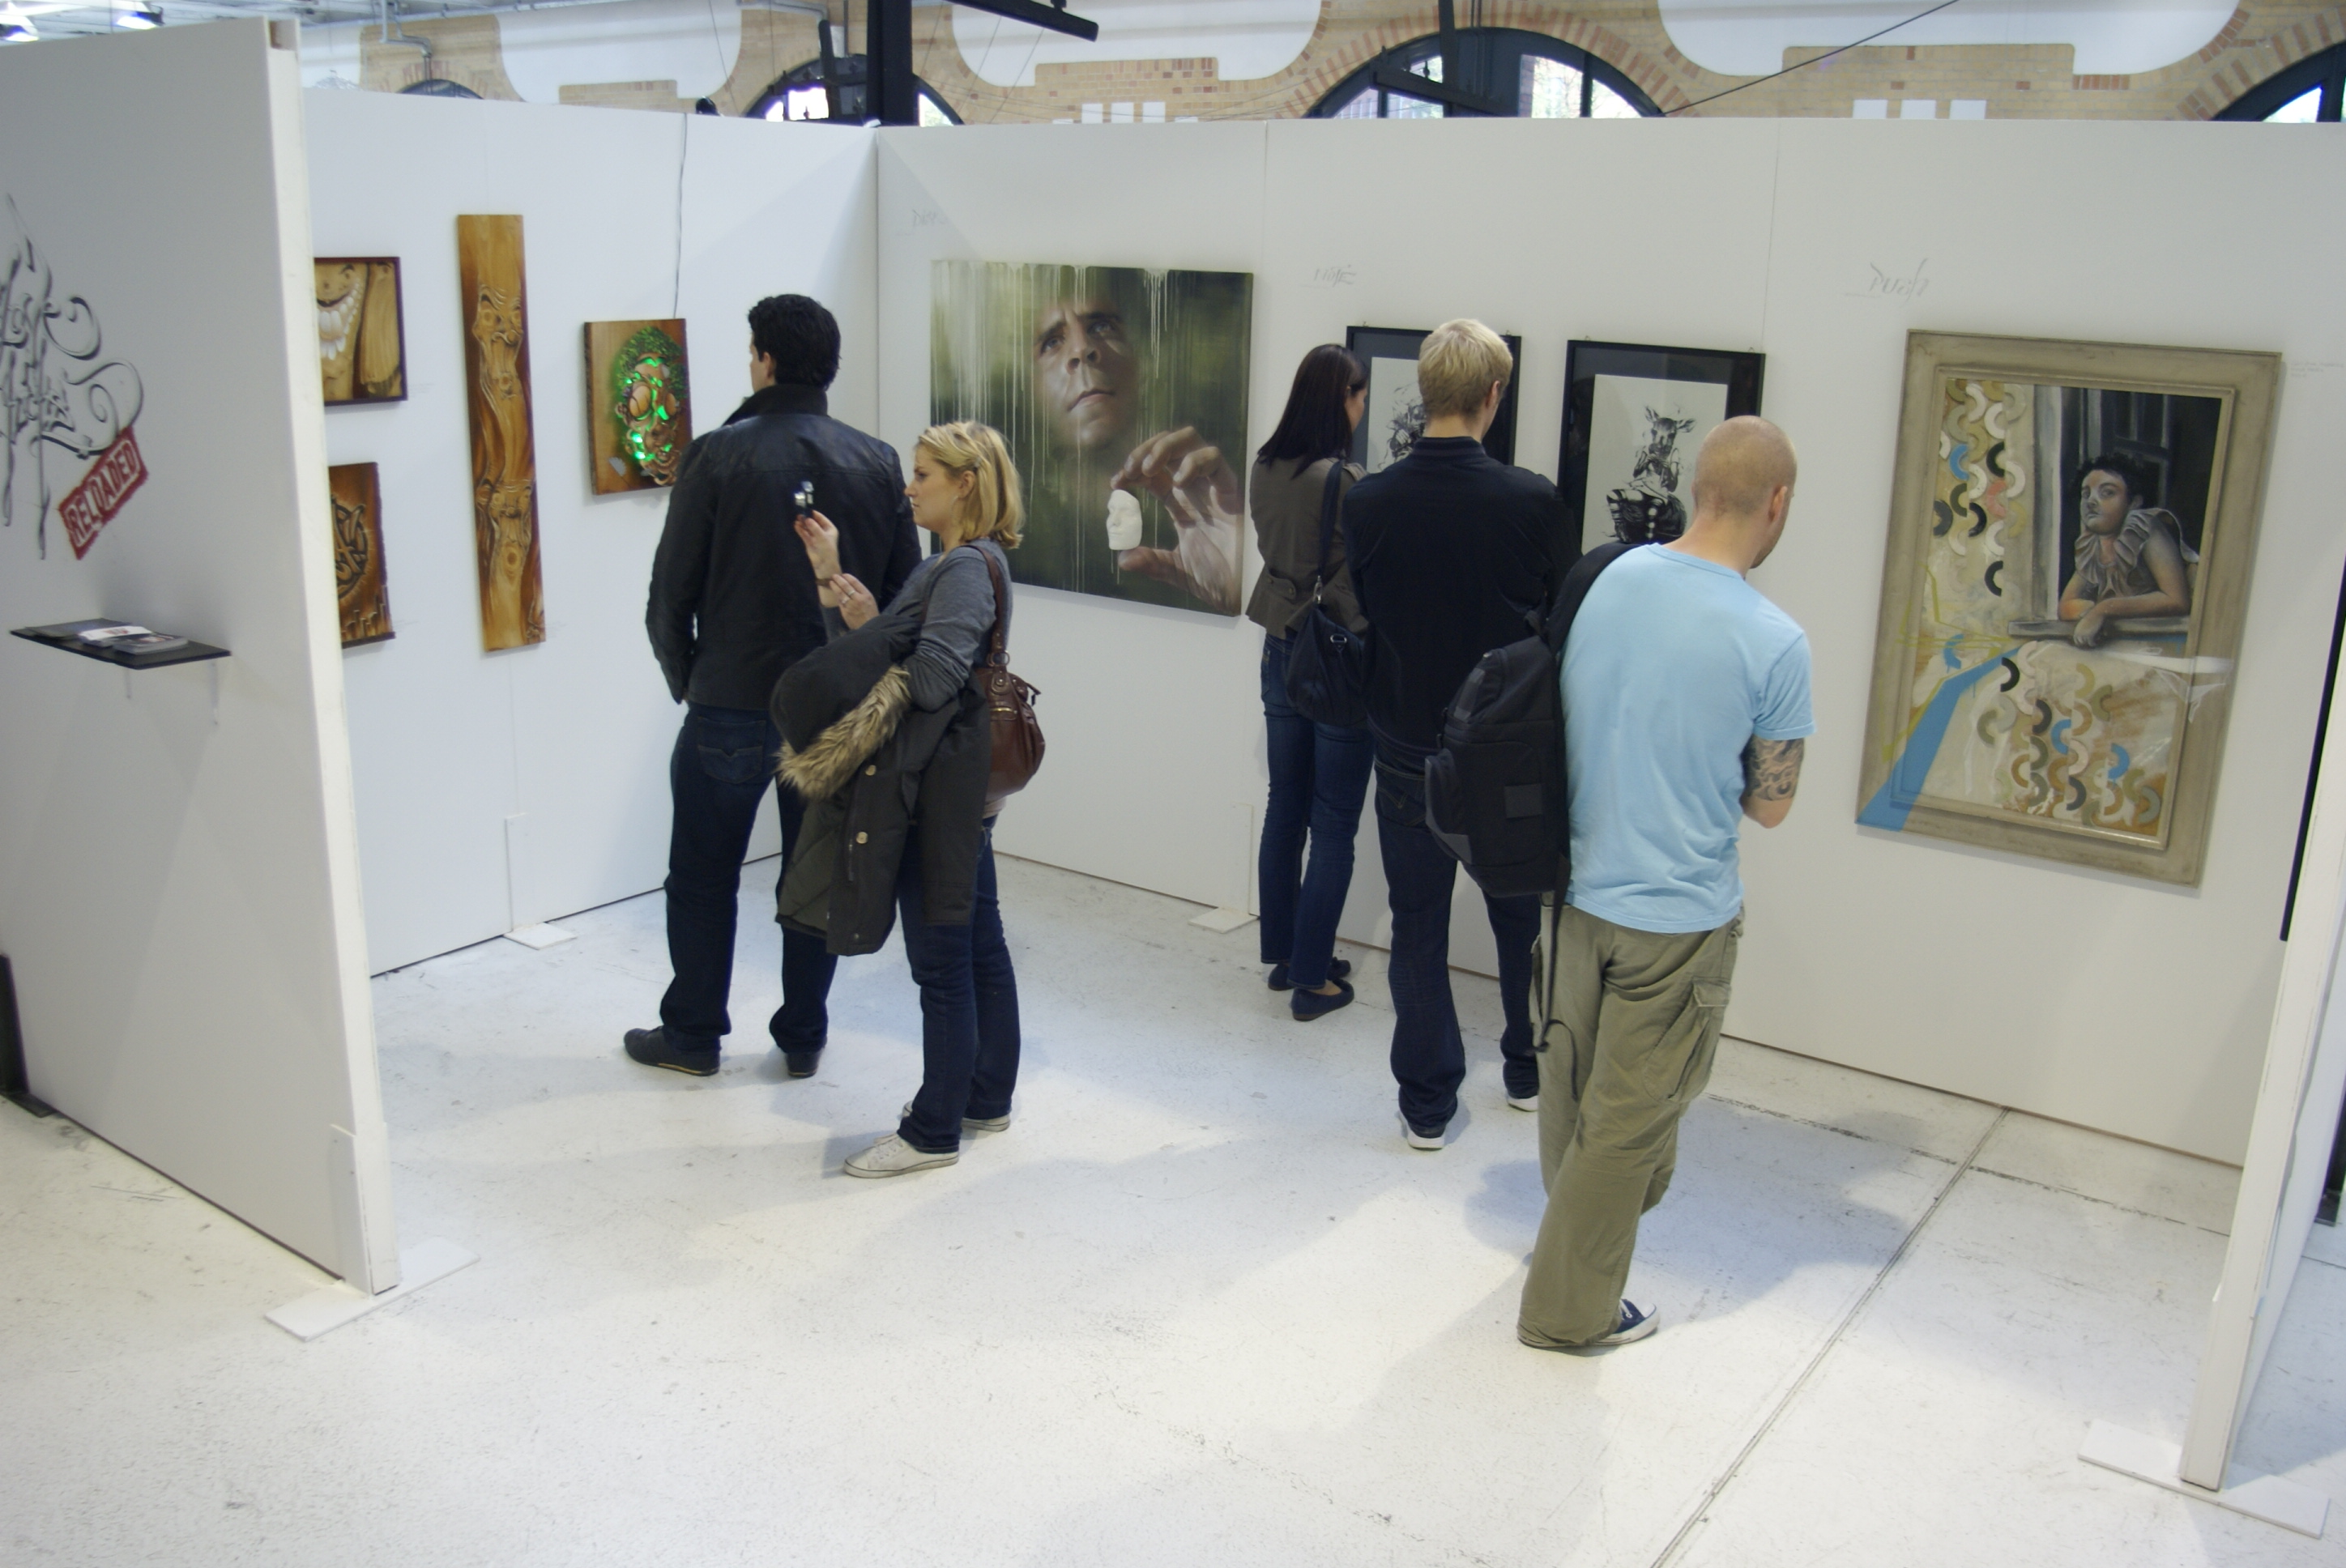
\includegraphics[width=0.8\textwidth]{Graphics/stroke}
	\caption[Stroke06-Ausstellung,  \url{http://www.stroke-artfair.com/deutsch/presse.html}]{Die letzte Stroke-Messe lockte viele Besucher an}
\end{figure}
Ich bin jedoch der Meinung, dass die N�he zur Illegalt�t und das Platzieren von Werken auf der Strasse Street-Art ausmachen. Galerien versuchen dies einzubinden. Banksy gelingt dies relativ gut in dem er Galerien nutzt, um Dinge zu zeigen die auf der Strasse nicht m�glich w�ren, wie zum Beispiel bemalte, lebendige Tiere.\footnote{\cite[Minute 49]{banksy2010}}. Auch vernachl�ssigt er die Arbeit im �ffentlichen Raum nicht, sondern nutzt die Stadt immer noch als sein Haupt-Medium. Das ist ihm hoch anzurechnen, da es nat�rlich bequemer ist seine Arbeit gem�tlich im Atelier zu erledigen, vor allem wenn sie so hohe Summen einspielt.



%************************************************
\chapter{Schlusswort}
\label{chp:schlusswort}
%************************************************

Zusammenfassend kann man sagen, dass Street-Art noch nicht im etablierten Kunstbetrieb angekommen ist. Dies ist darauf zur�ckzuf�hren, dass die Street-Art-Szene sich nicht aus traditionellen Kunstformen herausgebildet hat, sondern aus einer Subkultur stammt, die die Kapitalformen anders gewichtet als der etablierte Kunstbetrieb. Dazu kommt, dass die Street-Art als angewandte Kunst gilt, und auch deshalb vom Kunstbetrieb nicht anerkannt wird. Auch das Verhalten und der Habitus der Street-Art-Bewegung ist mit der hochkulturellen Kunstwelt nicht kompatibel. Es gibt zwar Ans�tze, mit Ausstellungen und Galerien Street-Art-K�nstler in den kommerziellen Kunstmarkt zu bef�rdern, dies ist jedoch sehr schwierig zu bewerkstelligen ohne dass man die Street-Art und damit die illegale Kunst im �ffentlichen Raum verl�sst. Doch Banksy zeigt, dass es m�glich ist, den Spagat zwischen Strasse und Galerie zu meistern. Es bleibt nun abzuwarten ob es weitere K�nstler schaffen werden. Die Bewegung der Street-Art ist sehr lebendig und es entstehen jeden Tag tausende neue Werke im �ffentlichen Raum. Auch die Street-Art-Ausstellungen vermelden steigende Besucherzahlen. Ich bin gespannt wie sich dies n�chster Zeit entwickeln wird, denn Street-Art hat definitiv das Potential, eine neue kunsthistorische Epoche zu werden.




% *****************************************************************
% Backmatter
%******************************************************************
\clearpage
%*******************************************************
% Bibliography
%*******************************************************
\nocite{*}
\printbibliography
%\vfill
\clearpage

%*******************************************************
% List of Figures
%*******************************************************    
%\pdfbookmark{Abbildungsverzeichnis}{abbildungsverzeichnis}
%\refstepcounter{dummy}

\begingroup 
    \let\clearpage\relax
    \let\cleardoublepage\relax
    \let\cleardoublepage\relax
    \phantomsection 
%    \refstepcounter{dummy}
		\addcontentsline{toc}{chapter}{\tocEntry{Abbildungsverzeichnis}}
		%\chapter*{Abbildungsverzeichnis}
    \listoffigures
    \vspace*{8ex}
\endgroup
\cleardoublepage


%*******************************************************
% Anhang
%*******************************************************
%\pdfbookmark[0]{Anhang}{Anhang}
\clearpage

\begingroup 
    \let\clearpage\relax
    \let\cleardoublepage\relax
    \let\cleardoublepage\relax
    \phantomsection 
%    \refstepcounter{dummy}
		%\addcontentsline{toc}{chapter}{Anhang}
		\begin{appendix}
		\chapter{Anhang}
		\section{Interview mit Seifrei}
				
[Wir treffen uns im Restaurant Drei Eiben im Gundeli. \emph{Seifrei} bringt seinen Kollegen Johannes mit und wir bestellen uns alle etwas zu trinken]
\bigskip
\\
\emph{Wie lange machst du schon Streetart, seit wann bist du etwa dabei?}
\\
Meine erste Schablone habe ich im �03 gemacht. �99 fing an ich mit sprayen, normal Graffiti halt. Streetart dann so richtig im �04/�05, also ungef�hr 8 Jahre.
\bigskip
\\
\emph{Wie bist du auf Graffiti und dann sp�ter auf Street-Art gestossen?}
\\
Also ich komme ja aus dem Webertal, und dort oben ist ja die Hip-Hop-Szene fest verankert. Und dann durch das ging ich halt mit den Jungs sprayen, dann bin ich durch das in die Graffitiszene hineingerutscht. Da ich nie gut Gesichter malen konnte, entdeckte ich im Ace \footnote{Ace Records, Graffiti und Hip-Hop-Laden in Basel} ein kleines Banksy-B�chlein, und habe das gekauft. Das hatte halt schon Einfluss, ich dachte: �Ha, voll geil, wenn man so eine Schablone machen und dann sprayen kann, warum lang Zeit brauchen wenn man schnell die Schablone hinhalten und dann sprayen kann.�. Durch das bin ich dann eben [in die Street-Art-Szene] hineingerutscht. Bin auch fast einmal von der Polizei erwischt worden, weil ich immer so langsam war
\bigskip
\\
\emph{Also damit ja �hnlich wie Banksy, der auch zuerst in der Writer-Szene aktiv war, und dann auf Schablonen umstieg, weil das viel schneller geht.}
\\
Ja, das ist halt eben einer der Hauptvorteile der Schablonen, die Schnelligkeit
\bigskip
\\
\emph{Was motiviert dich dazu Street-Art zu machen? Es ist ja meistens Nacht, du bist auf der st�ndigen Flucht vor der Polizei....}
\\
Neinnein, es geht mehr um den kreativen Teil, die Stadt zu gestalten, mitzugestalten, etwas lustiges von sich in der Stadt zu sehen, oder auch nicht. Es geht auch um die Aktion selbst an sich, das ist auch immer sehr witzig. Hmm, was gibt es noch..einfach mitgestalten und etwas aktiv machen, und halt die Sachen selbst sehen, und vielleicht auch um mal die Reaktion von den Leuten sehen, die an [einem meiner Werke] vorbeilaufen. Das sind so die Hauptgr�nde. Es macht auch Spass die Schablonen zu schneiden, teilweise sehr, und dann halt die Aktion draussen f�r sich, Adrenalin nicht unbedingt der Hauptgrund, aber ist lustig manchmal, obwohl das eher negativ ist, ich habe damit eher negative Erfahrungen gemacht.
\bigskip
\\
\emph{Ja genau, zu dem komme ich sp�ter nochmals. Siehst du deine Kunst eigentlich als Medium einer Botschaft?}
\\
�hh, nicht zwangsl�ufig.
\bigskip
\\
\emph{Also geht es eher um die Aktion selbst, oder hast du auch politische Motive?}
\\
Nein, nicht gross. Ab und zu vielleicht, ich machte einmal einen Araber, als dort die Revolution war.
\bigskip
\\
\emph{Ja, den habe ich gesehen!}
\\
Aber eigentlich [mache ich] nichts wirklich politisches, es geht mehr um Gesichter, und mehr um Emotionen die ich wecken will als eine Botschaft weiterzugeben.
\bigskip
\\
\emph{Also deine Kunst ist eher eine pers�nliche Ausdrucksart auf der Strasse.}
\\
Ja, ja genau, nein eine Botschaft eher nicht, mehr f�r die Sache selber, ��l�art pour art�, so irgendwas.
Oder ob es das ist, wie auch immer, ich sehe es auch nicht wirklich als Kunst, sondern eher als Aktivismus. Es geht auch darum, selber mitgestalten und nicht gestalten lassen, vom Architekt der Stadtverwaltung und den Werbefirmen. Es soll auch ein bisschen Gegenkontrast bieten. Werbung ist auch �berall penetrant und es fragt mich niemand ob ich �berhaupt das Riesenblitzlicht vom Mediamarkt sehen will wenn ich �ber die Bahnhofspassarelle laufen muss
\bigskip
\\
\emph{Den Raum der Stadt f�r sich also beanspruchen nach dem Motto: �Reclaim the Streets�}
\\
Genau, genau... ganz genau
\bigskip
\\
\emph{Verkaufst du deine Kunst oder machst du Auftragsarbeiten?}
\\
Beides eigentlich. Ich bin nicht darauf angewiesen dass ich davon leben muss, oder davon Leben will. Ich habe ein, zwei Orte wo ich Sachen verkaufen kann, ab und zu auch Ausstellungen, das sind meistens zwar so Gruppenausstellungen. In Amsterdam hatten wir das jetzt schon zweimal. Aber viel verkaufe ich dort eigentlich nicht, und auch im Netz [Internet] nicht. Jetzt habe ich ein paar Auftr�ge, die ab und zu reinkommen, aber eigentlich, wenn man die Bilanz anschaut, habe ich sicher 10-20 Tausend Franken f�r [Spray-]Dosen und alles ausgegeben.
\bigskip
\\
\emph{W�rdest du gerne davon leben, oder ver�ndert das den Charakter der Kunst?}
\\
Es ver�ndert auf jeden Fall den Charakter habe ich das Gef�hl, denn du musst dann alles machen, 
jeden Scheissjob, wo du im Normalfall w�rdest sagen: �Nein, da h�tte ich jetzt nicht so Lust drauf�, 
Klar, man kann's dann den ganzen Tag machen, sein Hobby, aber der Charakter �ndert sich sicherlich wenn man davon Leben k�nnen muss. H�chstens du bist wirklich gut, und kannst dann so exklusive Sachen machen, das du dann trotzdem deine eigene Sache durchziehen kannst. Dann hast du auch k�nstlerische Freiheit und musst nicht einen Schriftzug f�r irgendeine Bierfirma designen. 
\bigskip
\\
\emph{Wenn du die M�glichkeit h�ttest, von deiner Kunst zu leben, w�rdest du das tun, oder w�rdest du es immer als Hobby durchziehen?}
\\
Ich glaube wenn ich k�nnte, w�rde ich schon, aber erstens wird man nicht wirklich reich davon, und zweitens muss man dann halt wirklich alles machen, wie gesagt, ich denke nicht das ich es je machen w�rde, ich habe dann vielleicht einen Job der mir gef�llt, mehr oder weniger, und [Street-Art] nebendran als Ausgleich und sonst halt das Leben geniessen, so ist eher der Plan.
Ob es f�r mich reichen w�rde [ganz selbstst�ndig zu werden], w�sste ich jetzt nicht, habe mir die Frage eigentlich noch nie so gestellt, der Markt in der Schweiz hier ist fast zu klein als dass man davon richtig gut leben kann. Lieber eine gute Ausbildung und ein guter Job.
\bigskip
\\
\emph{In letzter Zeit erhielt Street-Art, unter anderem durch Banksy, immer mehr �ffentliches Interesse, auch die Zahl der Austellungen und Galerien die Street-Art ausstellen nahm zu. Wie stehst du dazu, 
ist dieses �ffentliche Interesse gut f�r die Street-Art-Szene, oder soll Street-Art eine Underground-Subkultur bleiben?}
\\
Es ist ein bisschen ambivalent, es gibt beide Seiten. Es ist sicher sch�n, wenn [Street-Art] Aufmerksamkeit bekommt und auch in den Medien und renommierten Galerien auftaucht. Es kommt immer drauf an was man unter Street-Art versteht, und wer diese Street-Artists sind, die dort ausstellen. Zum Teil sind es Leute, die schon lange nichts mehr auf der Strasse machen, und dann halt unter dem Label der Galerie sich durch alle Ausstellungen durchboxen. Auf der anderen Seite hats dann auch so Leute wie der C215, die halt voll krass auf der Strasse sind, und dann nebenbei viel Ausstellungen machen und dann dadurch viel Aufmerksamkeit bekommen, das finde ich super. Aber es wird dann schnell auch ein bisschen Sell-Out m�ssig, es gibt viele Leute, die dann nur noch in den Galerien sind. Und dann kommen jene Grosskonzerne, Mini, BWW und alle wollen sich ein St�ck von dem abschneiden und diese Leute machen dann irgendwelche Live-Events und Performances, wo dann immer die Frage im Raum steht, was machst du da mit Street-Art, du spannst es f�r irgendein Produkt ein, ob du dann dahinter stehen kannst, ist dann vielleicht eine andere Sache.
Es ist dann schon eher in Richtung Ausverkauf gegangen mit dieser Aufmerksamkeit [um Street-Art].
Das ist eher wieder ein bisschen am abflauen, habe ich das Gef�hl. In der Graffiti-Szene geschah anfangs, oder eher Mitte-80er ein �hnliches Ph�nomen, da sind pl�tzlich auch alle in Galerien aufgetaucht. Das ist tempor�r habe ich das Gef�hl. Es ist sicher nicht schlecht, aber es beschleunigt auch den Sell-Out.
\bigskip
\\
\emph{Was bezeichnest denn du als Sell-Out? Ist das einfach, wenn man alles f�r Geld macht oder...}
\\
Nein, also wenn man sagt, man ist Street-Artist, dann arbeitet man, von mir aus gesehen, haupts�chlich auf der Strasse. Man macht sein Zeugs draussen, vielleicht geht�s kaputt, vielleicht auch nicht. Aber wenn die Leute dann nur noch von Galerie zu Galerie gehn', und dann vielleicht nur noch ein Bild pro Jahr machen, wenn sie �berhaupt noch auf der Strasse sind, dann ist das f�r mich nicht mehr Street-Art, sondern irgendwie etwas anderes, weiss doch auch nicht wie man es dann nennen will, das ist noch eine schwierige Definitionsfrage.
\bigskip
\\
\emph{Du hast am Anfang kurz Banksy anget�nt, was h�ltst du von ihm, viele Leute bezeichnen ihn ja auch als Sell-Out, er verkauft seine Sachen nur noch, doch er versucht immer noch, unerkannt zu bleiben und auch einen Mythos um seine Person zu machen, wie stehst du dazu?}
\\
 Also ich finde sein Zeugs super, was er macht. Also erstens wollte er das nie, dass er so ein Sell-Out wird, und zweitens nervt ihn das selber extrem, er macht sich ja auch �ber das lustig, mit seinen neuen Sachen, und drittens, finde ich, seine Sachen, die er macht, sind immer sehr ironisch, muss immer lachen wenn ich seine Sache seh, und es ist auch sch�n gemacht, auch die Locations und so. Also ich finde ihn super. Es ist immer cool, frische Sachen von ihm zu sehen. Das Sell-Out ist ein Nebenprodukt, was er nicht unbedingt hat wollen, klar ist es cool wenn man in L.A f�r �ber eine Million Zeugs verkaufen kann, und den reichen Trottel sein Zeugs andrehen kann. Aber er hat es glaubs nie so wollen, oder so geplant, aber es ist herrlich dass es so herausgekommen ist, es ist cool dass er noch so viel macht und er hat jetzt wirklich schon viele Projekte angerissen.
\bigskip
\\
\emph{Also er ist in dem Sinn kein Sell-Out, da er immer noch aktiv auf der Strasse ist, und nicht nur noch in den Galerien t�tig ist.}
\\
Genau.
\bigskip
\\
\emph{Das haben wir vorher noch kurz angesprochen, spielt die Illegalit�t bei Street-Art eine Rolle?}
\\
Also es geh�rt schon dazu, es ist auch immer ein Machtkampf, irgendwie auch, zwischen denen, denen die W�nde geh�ren, den Immobilienbesitzer, den Werbefirmen, der Stadtverwaltung, und denen die kommen, und einfach [Street-Art] machen. Wegen dem ist die Illegalit�t sicher wichtig, solange die Stadt die Fl�chen nicht f�r alle freigeben.
\bigskip
\\
\emph{W�rdest du lieber alles legal machen, also wenn du jetzt W�nde zur Verf�gung gestellt bekommen w�rdest, die immer noch auf der Strasse sind, w�rdest du das lieber machen?}
\\ 
Nur wenn sie alle W�nde freigeben w�rden, sonst nicht. Es geh�rt dazu, weil die Besitzverh�ltnisse jetzt nun mal so sind. Auch wenn alle W�nde f�r Street-Art freigeben w�ren, geh�rt es dazu, den Ort auszuw�hlen, es ist sehr wichtig, wo man es macht.
\bigskip
\\
\emph{Oft wird ja Street-Art im selben Atemzug wie Graffiti erw�hnt. Street-Art hat sich aus der Graffiti-Szene herausgebildet, bildet Street-Art nun eine eigene Szene, inwiefern unterscheiden sich die beiden?}
\bigskip
Ja, das	 ist eine schwierige Frage, da k�nnte man stundenlang dar�ber reden. Graffiti ist halt mehr ein bisschen, hmm wie soll ich das sagen, es geht  mehr um das zerst�rerische , denn  Z�ge bemalen ist dort das gr�sste, und �berall in der City was machen, und auch das ganze mehr mit der Crew. Bei der Street-Art-Szene, also die Schablonen-Typen, Paste-up-Typen, die sind nie so fest in Crews organisiert wie�s die Writer sind. Es gibt es zwar auch, aber nicht annh�hernd so ausgpr�gt. Graffiti gibt es ja auch schon ein bisschen l�nger, aber es gab auch fr�he Street-Artists, wie Blek le Rat. Es halt schon eine  v�llig andere Szene, w�rde ich sagen. Ein Kollege sagte das sch�n: �Same game, different players�. Es ist halt schon der gleiche Grundgedanke dahinter.
\bigskip
\\
\emph{Graffitikunst ist bis jetzt, oder vor allem in letzter Zeit, nicht mehr so im Rampenlicht der Medien und Kunstgalerien gewesen und auch nicht  so kommerziell erfolgreich auf dem Kunstmarkt wie Street-Art. An was k�nnte das liegen?}
\\
Ich habe das Gef�hl das dass bei Street-Art auch wieder  hinuntergehen wird, dieser Boom. Der wird ganz klar an Aufmerksamkeit einb�ssen. Klar, Street-Art ist halt noch mehr mit dem Grafischen �berschnitten, und so Sachen, die machen auch Drucke und so, das spricht die Leute halt mehr an.
Bei Graffiti gibt es so viele die es machen, und die Leute sehen es so oft, doch die sehen meist kaum, ob das jetzt einer ist, der gut ist oder nicht. Es ist schon eher von der Szene f�r die Szene, ein normaler Zugfahrer schaut nicht jedes mal beim durchfahren die Line [Bahnlinie] an und schaut wie sie jetzt frisch aussieht. Es sind auch die Schriftz�ge, die die Leute nicht ansprechen, das sind ja Hieroglyphen f�r die meisten Leute. 
Wenn du nat�rlich Gesichter oder andere Installationen machst, ist das viel ansprechender f�r den Normalb�rger, als wenn er einen f�r ihn unleserlichen Schriftzug sieht, und daneben einen ebenso f�r ihn unleserlichen Tag, und noch ein paar Farben dazu. Oder auch nur Chrom und Schwarz. Von dem her ist es eigentlich klar das [Street-Art] ansprechender ist f�r die Leute. In den 80er gab es eben den genau gleichen Boom um Graffiti und das wird bei Street-Art meines Gef�hls nach auch wieder zur�ckgehen. 
Aber wir werden es ja sehen, mal schauen.
\bigskip
\\
\emph{Vielen Dank Seifrei f�r dein Interview!}
\\
 Ja, ich hoffe ich konnte dir etwas brauchbares liefern!
\cleardoublepage

\section{Interview mit Bust}
Ich tauschte mich mit dem Basler Streetartist Bustart, der momentan in Amsterdam wohnt, per E-Mail aus.
\bigskip
\\
\emph{Was heisst f�r dich Street-Art, wo f�ngt es an und wo h�rt es auf?}
\\
Mir pers�nlich passt der Name "`Street-Art"' �berhaupt nicht, denn dieser nennt jede Ver�nderung im �ffentlichen Raum Kunst, was in meinen Augen nicht unbedingt stimmt. Street-Art kann fr�hlich sein, traurig, politisch, lustig oder auch nichtssagend, in den seltesten f�llen ist es Kunst. Ich finde dies h�ngt nur vom betrachter ab und seiner Einstellung gegen�ber dieser "`Kunst"' \\
Das Wort Street-Art gibt es seit 2004 dank dem Woostercollektive\footnote{Ein amerikanisches Street-Art-Archiv und Street-Art-Blog, \url{http://woostercollective.com}}, dort wurde abgestimmt wie diese Form sich im �ffentlichen Raum auszudr�cken heissen soll.
\bigskip
\\
\emph{Wie lange machst du schon Steet Art?}
\\
Ich habe 1999 mit Graffiti angefangen und mache seit 2005 aktiv Street-Art.
\bigskip
\\
\emph{Wie bist du auf Street-Art gestossen und was hat dich dazu bewogen anzufangen, beziehungsweise weiterzumachen? }
\\
Ich habe das Buch "`The Art of Revolution"' in die Finger bekommen und habe mich extrem am�siert, die Arbeiten haben mich mehr bewegt als klassisches Graffiti. Der Hauptgrund war wohl, dass es das in Basel nicht gab. Es gab sehr wohl schon eine aktive K�nstlerin namens "`bird"' sie hat etliche Sticker in Basel geklebt meist mit Karl dem Grossen drauf, oder einem Ohr. Ich habe diese Sticker mehr so als Propaganda gesehen. Auf jedenfall gab es sowas wie Schablonen, Poster oder Installationen nicht wirklich.
\bigskip
\\
\emph{Was motiviert dich Street-Art zu machen?}
\\
Gute Frage, ich denke jeder Mensch hat seine Berufung, ich seh mich selbst als K�nstler; die Strasse ist meine Galerie und mit dem was ich mache dr�nge ich den Leuten auf der Strasse ungefragt meine Kunst auf. Ob es der grossen Masse gef�llt ist mir egal. Sogesehen ist es eine sehr egoistische Art mich auszudr�cken.
\bigskip
\\
\emph{Kannst du von deiner Kunst leben?}
\\
Nein leider noch nicht.
\bigskip
\\
\emph{Wenn ja, musst du auch Auftr�ge annehmen, die dir nicht gefallen um dich finanziell �ber Wasser halten zu k�nnen?}
Hmm, ich habe sehr wohl schon das ein oder andere gemalt, was ich im Nachhinein bedauert habe, dann aber nur weil ich nicht bezahlt wurde oder nur halb, im Grossen und Ganzen will jeder etwas gemalt haben, aber nur sehr selten ist jemand bereit auch daf�r zu bezahlen.
Wenn man versucht von dieser Kunst zu leben ist es immer schwer abzuwiegen, ob man den Auftrag annimmt um ein paar Euro zu verdienen oder ablehnt weil man sich unterbezahlt f�hlt.
\bigskip
\\
\emph{Street-Art hat in letzter Zeit international erh�hte Aufmerksamkeit erhalten, ist das gut f�r dich als Street-Artist  geht da ein bisschen der Underground-Subkultur-Aspekt von Street-Art verloren?}
\\
Jein. Street-Art wurde sehr schnell kommerziell, einige wenige verdienen ein Arsch voll Geld und dies wird in den Medien verbreitet, darum denken einige hier geht es um schnelles Geld. In Wirklichkeit gibt es aber in jeder Stadt nur sehr wenige wirklich aktive K�nstler, zum Beispiel: Basel 3-4, Z�rich 4-5, Bern 2-3, und Amsterdam hat etwa 5-6.
\bigskip
\\
\emph{Mit Banksy gab es ja fast einen richtigen Street-Art Boom. Wird dieses mediale Rampenlicht anhalten, oder wird Street-Art langsam wieder an Aufmerksamkeit verlieren und zum selben Punkt wie vor etwa Zehn Jahren zur�ckkehren?}
Das weiss ich nicht. Es gab den selben Boom ja auch in den 80gern mit Graffiti, nur diesmal kann die breite Masse etwas mit den Motiven anfangen. Wer weiss was als n�chstes kommt.
\bigskip
\\
\emph{Was m�sste sich im etablierten Kunstbetrieb �ndern, damit Street-Art sich besser in den offiziellen Kunstmarkt integrieren k�nnte?} \\
Es ist immer schwer, zeitgen�ssische Kunst an den Mann zu bringen, die meisten K�nstler werden nach ihrem Tod ber�hmt. Ich sehe Graffiti und Street-Art als neue Kunstepoche nach Popart. Es gab weltweit noch nie eine so grosse Bewegung und Netzwerke wie �ber diese Kunstform.
\\
Doch der Wert wird immer noch vom K�ufer bestimmt.
\bigskip
\\
\emph{Inwiefern m�sste sich die Street-Art ver�ndern, um besser von der Kunstgesellschaft aufgenommen zu werden und k�nnte man das dann noch als Street-Art bezeichnen?}
\\
Ich denke, Street-Art geht schon viel zu sehr in diese Richtung und verliert so seine Seele. Es geht f�r mich immernoch um den Kontakt mit anderen Leuten auf der Strasse, ein gutes Bild auf der Strasse ist 100 mal mehr Wert als ein Foto einer Leinwand in einem Katalog.
\bigskip
\\
\section{Interview mit c215}
Ich tauschte mich per E-Mail mit c215 aus.
\bigskip
\\
\emph{Where are you from and what did you do before making Street-Art} \\
I'm from Paris. I've always been drawing and I painted in the street with a spray bomb for the first time almost twenty years ago. It already was �vespas� of a real size and I still paint them today, but with stencils not on �free hand� anymore � I have 35 of them. I followed university studies in art history, until a PhD at the Sorbonne. Things only became serious little by little.
\bigskip
\\
\emph{What�s Street-Art for you, where does it start and where does it end?} \\
Street-Art is only urban collective poetry.
\bigskip
\\
\emph{What makes Street-Art different from graffiti?} \\
Graffiti is mainly marking his name with style in the city while Street-Art is more aiming at transforming contextual situations in a defined architecture.\bigskip
\\
\emph{How did you get into Street-Art?} \\
Through my daughter, I painted her portrait in her district when she was a little girl.
\bigskip
\\
\emph{Her portrait is now all over the world. How did she react to this?} \\
At the beginning she was not interested, but the more she grows the more she is involved in the process. She�s a real stencil artist now and she is able to do two layers pretty well.	
\bigskip
\\
\emph{What motivates you getting up on the street, considering it would be much easier to just do indoor work?} \\
Painting on a canvas is boring, it's much more exciting to paint outside without authorization. Outside there's no mediation as well.
\bigskip
\\
\emph{Do you live off Street-Art? If not, would you like to?} \\
I am living as an artist.
\bigskip
\\
\emph{Do you think a Street-Artist has it harder to get the attention of galeries and such as a conventional contemporary artist?}\\
Street-Artists looking for galleries are a stupid and have the wrong ideals. The best gallery is the street.
\bigskip
\\
\emph{Does selling your work affect you or your art?}\\
Nothing is changing my art. I don't care about influence of the market
\bigskip
\\
\emph{Do you think the attention Street-Art got through Banksy will decline in future?} \\
Yeah like Rock n Roll was said to have no future in the 50's and it has just changed the world and provided the biggest ideology of 20th century. So no, I don't think so.
\bigskip
\\
\emph{What do you think could help Street-Art reaching a wider audience and getting shown more by galerists and in established art shows?} \\
Oh my god, you're so obsessed about galleries. Such a boring subject.
\bigskip
\\
\emph{What are the chances of seeing your work in Switzerland anytime soon? You�re always welcome!} \\
I may come this spring to Zurich

	
%\section{Interview mit Rik Reinking}
%Ich interviewte Rik Reinking per E-Mail.
%\bigskip
%\\
%\emph{Was ist f�r der Unterschied zwischen Graffiti und Street-Art?}\\
%Ich glaube, der bessere oder treffendere Begriff f�r diese gegenw�rtige Bewegung w�re Urban Art. Also Kunst, die ihre Wurzeln im Urbanen � im Stadtraum � hat. Street-Art und Graffiti sind Spielarten und Ausdrucksformen dieser Bewegung. Dabei versteht man unter Graffiti �Malen� mit der Spr�hdose. Street-Art zeigt sich eher in Form von Stickern, Plakaten und Paste-Ups\footnote{Paste-Ups sind mit Kleister oder Leim aufgezogene Plakate, die mit vorher mit Schablonen bespr�ht oder von Hand bemalt wurden}.
%\bigskip
%\\
%\emph{Du bist Kunstsammler und besitzt auch viel Street-Art. Was fasziniert dich daran?}\\
%Ich f�hle mich von dieser Kunst verstanden und ich kann mich in dieser Kunst f�hlen. Es entspricht meiner Generation � und �hnlich wie beim Fluxus\footnote{Eine sehr radikale und experimentelle Kunstbewegung in den 60ern, die sich gegen die konventionelle Kunst richtete} verl�sst diese Kunst das Museum und den Ausstellungsraum. Jetzt gibt es eine Generation, die im �ffentlichen Raum aufgewachsen ist, im �ffentlichen Raum Kunst gemacht hat und diese wieder in den musealen Kontext bringt. Dabei sind viele Positionen von jungen, zeitgen�ssischen Street-Artists �hnlich wie bei David Hammons, Alan Kaprow und vielen Fluxus-K�nstlern � und das fasziniert mich.
%\bigskip
%\\
%\emph{Du giltst ja als einer der ersten Street-Art-Sammler. Wie hat sich die Street-Art-Szene seit damals ver�ndert?}\\
%Die Arbeiten sind viel teurer geworden, es gibt viele Kunstwerke, die ich mir nicht mehr leisten kann. Aber ich finde das ganz am�sant. Vor einigen Jahren gab es noch viele, die mich f�r genau diesen Teil meiner Sammlung ausgelacht haben. Und die kommen jetzt angerannt und fragen mich um Rat, wo sie noch Street-Art kaufen k�nnen. Aber das ist mir alles v�llig egal, denn Trends interessieren mich nicht. Ich hatte den Dialog mit den K�nstlern vor 10 Jahren und ich habe ihn noch heute. Und mit einigen wird es einfacher, mit anderen schwieriger. Es h�ngt davon ab, wie sich ein K�nstler positioniert und wie sehr er sich vom Kunstmarkt verreinahmen l�sst. Manchen steigt der Ruhm und das Geld schon sehr zu Kopf.
%\bigskip
%\\
%\emph{Von welchen K�nstlern sind die Preise denn so stark angestiegen zum Beispiel?}\\
%Banksy, Os Gemeos, Swoon, Zevs und Daim sind unglaublich teuer geworden.
%\bigskip
%\\
%\emph{Du hast viele dieser K�nstler in deiner Sammlung und hast sie auch schon ausgestellt. Hast du diese K�nstler teilweise auch selbst gross gemacht?}\\
%Nein. Swoon und Os Gemeos werden zum Beispiel jetzt auch von Deitch vertreten, einem m�chtigen New Yorker Galeristen. Aber das sind auch alles K�nstler, die konsequent und verantwortungsbewusst mit ihrem Werk umgeben. Und ich sammle diese K�nstler, weil ich sie auch am l�ngsten beobachte und mit ihnen auch am meisten zu tun habe. Es w�re ja komisch, wenn ich nur Kunst sammeln w�rde, die erst seit einem halben Jahr ein Thema sind. Das ist ganz nat�rlich gewachsen. Street-Art bestimmt seit vielen Jahren meinen Alltag und ich habe auch meine Freunde in diesem Bereich.
%\bigskip
%\\
%\emph{Warum ist ihrer Meinung nach das Interesse an Street-Art vom Kunstmarkt, Medien und Museen so stark gestiegen?} \\
%Weil alle sehen, dass Street-Art authentisch ist. Auf dem Kunstmarkt sehe ich dagegen nur wenig Authentisches. Auf Messen gibt es unglaublich viel Mist, der extra f�r den Kunstmarkt produziert wurde � oft im kleinen Format, damit man es sich gleich unter den Arm klemmen kann. Der Kunstmarkt wird nat�rlich aufmerksam, wenn er sieht, dass da etwas wirtschaftlich erfolgreich ist. Wenn die Nachfrage steigt, dann geht eben auch der Preis hoch. Und Museen haben erkannt, dass Street-Art Zeitgeschichte und ein Zeitdokument ist. Wenn wir in zehn Jahren zur�ckschauen, dann wird diese Zeitspanne historisch sein und auch die K�nstler, die in ihr gelebt haben. Viele Museen springen nat�rlich auf den Zug auf, weil sie in zehn Jahren die ersten sein wollen, die das bereits erkannt haben. Das sind Eitelkeiten. Und warum die Medien begeistert sind, ist klar: Diese Kunst kommt schon sehr lecker daher. Sie ist zug�nglich, denn sie will ja m�glichst viele Leute erreichen. Das ist ja keine Donald-Judd-Kiste, �ber die sich 90 Prozent der Besucher aufregen, denken "`Was soll der Schei�"' und ihr Bier darauf abstellen\footnote{Anm. Stefan: Donald Judd war ein Vertreter der Minimalismus-Kunstrichtung und stellte auch einfache Boxen aus, was f�r Aussenstehende oft nicht als Kunst betrachtet wurde, frei nach "`das kann doch jeder..."'}. Au�erdem ist Street-Art eine globale Bewegung. Auch beim Fluxus gab weltweit K�nstler, die eine gemeinsame Bildwelt und -sprache hatten. Mit verschiedenen Akzenten und jeder mit einer eigenen Handschrift, aber trotzdem gab es eine Gruppe und eine Bewegung. Dann kam lange, lange nichts � und heute gibt es Street-Art.
%\bigskip
%\\
%\emph{Denken Sie, die Aufmerksamkeit um Street-Art ist nur ein Trend und wird mit der Zeit langsam abflauen?}\\
%Das ist ja ein Spiel. Und das ist beim gesamten Kunstmarkt so: Preise werden k�nstlich noch oben gepumpt und dann l�sst man Preise wieder einbrechen. Von Auktion zu Auktion steigen die Arbeiten mit den Sch�tzungen. Die heutigen Auktionsh�user kann man alle vergessen, weil sie keinerlei Verantwortungsbewusstsein haben.
%\emph{Wie kann sich ein K�nstler l�nger auf dem Kunstmarkt bew�hren?}
%Verantwortungsbewusstsein dem eigenen Werk gegen�ber ist das Wichtigste. Wenn der K�nstler m�chte, dass man ihn Ernst nimmt, wenn er ein h�heres Preisniveau erreichen m�chte, dann muss er dem Preis, dem K�ufer und dem Markt gegen�ber verantwortungsbewusst sein. Es gibt K�nstler, die haben einen entspannten Umgang mit ihrem Werk, und denen ist das egal. Und andere sind an hohen Preisen interessiert. Aber ein hoher Preis sagt nichts �ber die Qualit�t einer Arbeit aus. Ich kenne fantastische K�nstler, die seit Anfang an dabei sind, und von denen kann man noch immer Originale f�r hundert Euro kaufen. Und dann gibt es K�nstler, die sind auf Auktionen richtig teuer. Aber ein Markt w�chst erst �ber die Zeit, es ist immer eine Frage von Angebot und Nachfrage. Das kann man jetzt noch gar nicht absehen. Manche werden wegbrechen, manche werden vielleicht einfach einen B�rojob annehmen, viele sind ja noch sehr jung. Aber andere werden weiter machen, weil sie gar nichts anderes machen k�nnen, die haben so eine unglaubliche Motivation und Energie.
%\bigskip
%\\
%\emph{Street-Art ist ja im Grunde auf der Strasse und ist eher tempor�r und verg�nglich, da es meist schnell wieder weggeputzt wird. Also sollte es ja eigentlich nur wenige Werke auf dem kommerziellen Kunstmarkt geben, oder?}\\
%Ja, es gibt wenig Authentisches. K�nstler wie Blu machen gar keine kommerziellen Geschichten. Wenn man Gl�ck hat, verkauft er einem eine Zeichnung aus seinem Skizzenbuch, und die sind dann auch wirklich sehr teuer. Aber das ist bei ihm das einzige, was man �berhaupt bekommt. Und das ist auch gut und konsequent so. Der lebt f�r die Sache. Und dann gibt es andere K�nstler, die bringen jeder Woche einen neuen Print oder eine Leinwand in Auflage heraus � das wird dann durchgespielt bis zum Umfallen. Ein wenig rar sollte man sich mit seinem Werk schon machen. Man kann nicht gnadenlos fluten und denken, das geht dann immer so weiter.
%
%\emph{Verliert Street-Art nicht seinen Reiz, wenn es pl�tzlich in Galerien und Museen auftaucht?}\\
%Nein. Es handelt sich dabei ja um v�llig unterschiedliche Arbeiten. Es gibt Arbeiten, die funktionieren nur im Innenraum, andere dagegen nur auf der Stra�e, und wieder andere funktionieren �berall. Und manche K�nstler besch�ftigen sich auch genau mit dieser Schnittstelle. Aber der Reiz geht dabei nicht verloren. Manche Arbeiten verlieren etwas und bei anderen Arbeiten kommt etwas hinzu. Aber da muss man sich frei machen � und eine illegale Arbeit im �ffentlichen Raum wird nat�rlich immer etwas v�llig anderes bleiben.
\end{appendix}

\endgroup
\cleardoublepage



%*******************************************************
% Deklaration
%*******************************************************
%\refstepcounter{dummy}
\pdfbookmark{Deklaration}{deklaration}

\begingroup
\let\clearpage\relax
\let\cleardoublepage\relax
\let\cleardoublepage\relax
\chapter*{Deklaration}
\thispagestyle{empty}
Hiermit erkl�re ich, Stefan Schneider, dass ich die Maturarbeit ohne fremde Hilfe 
angefertigt habe und nur die im Quellenverzeichnis angef�hrten 
Quellen und Hilfsmittel benutzt habe.
\bigskip
 
\noindent\textit{\myLocation, \myTime}

\smallskip

\begin{flushright}
    \begin{tabular}{m{5cm}}
        \\ \hline
        \centering\myName \\
    \end{tabular}
\end{flushright}
		

\vfill
\endgroup
\cleardoublepage

%\end{flushleft}
\clearpage
%%*******************************************************
% Index
%*******************************************************
\manualmark
\markboth{\spacedlowsmallcaps{\indexname}}{\spacedlowsmallcaps{\indexname}}
\phantomsection
\begingroup 
    \let\clearpage\relax
    \let\cleardoublepage\relax
    \let\cleardoublepage\relax
\pagestyle{scrheadings} 
\addcontentsline{toc}{chapter}{\tocEntry{\indexname}}
\
\endgroup 

\end{document}